\documentclass[a4paper,11pt,openany]{book}
\usepackage{knowledge}

\title{Математические основы криптологии}
\author{Автор курса: Применко Эдуард Андреевич \\ 
		Составитель: Смирнов Дмитрий Константинович}
\date{Версия от \currenttime, \today}

\begin{document}

\maketitle
\tableofcontents

\mainmatter
\chapter{Домашние задания}

\section{Теоретико-числовые методы и алгоритмы}

Задачи в этом разделе решаются со следующими параметрами:

\medskip

{\centering
\begin{tabular}{||c|c|c||}
\hline
\textbf{p} & \textbf{g} & \textbf{k} \\
\hline
23 & -8 & 22 \\
\hline
\end{tabular}

}

\medskip

\task{Убедиться, что $g \in \mathbb{Z}_p^*$ -- примитивный элемент $\mathbb{Z}_p$.}

Так как $p = 23$ -- простое число, то $\phi(p) = p - 1 = 22$. Разложим это число на простые множители: $\phi(p) = 2 \cdot 11$. Тогда достаточно проверить следующие 2 неравенства:
$$ g^{ \frac{\phi(p)}{2} } = (-8) ^ {11} = 15 \cdot 15 ^ {10} = 15 \cdot 18 ^ 5 = 17 \cdot 2 ^ 2 = 22 \not\equiv 1 \pmod p,$$
$$ g^{ \frac{\phi(p)}{11} } = (-8) ^ {2} = 18 \not\equiv 1 \pmod p,$$

Делаем вывод, что $g$ действительно является примитивным элементом $\mathbb{Z}_p$.

\task{Найти образующий элемент $h$ группы $\mathbb{Z}_{p^2}^*$}

Образующий элемент группы $\mathbb{Z}_{p^n}^*, n \ge 2$ имеет вид:
$$ h = g + t_0 p, \; t_0 \not \equiv g \nu \pmod p; \; \nu = ( \frac{ g ^ {\frac{p -1}{2}} + 1}{ p } )(\!\!\!\!\!\! \mod p) \cdot (-2)(\!\!\!\!\!\! \mod p)$$
\noindent Таким образом,
$$ \nu = ( \frac{ (-8) ^ {\frac{23 - 1}{2}} + 1}{ 23 } )(\!\!\!\!\!\! \mod 23) \cdot (-2)(\!\!\!\!\!\! \mod 23) = ( 1 \cdot (-2))(\!\!\!\!\!\! \mod 23) = 21$$
$$ t_0 \not \equiv (-8) \cdot 21 \!\!\!\pmod {23} = 16 \!\!\!\pmod {23} $$
$$ t_1 = 1 \Rightarrow h = (-8) + 1 * 23 = 15 $$
Следовательно, $h = 15$ -- образующий элемент группы $\mathbb{Z}_{23^2}^*$

\task{Подсчитать число образующих группы $\mathbb{Z}_{p^3}^*$}

Число образующих группы $\mathbb{Z}_{23^3}^*$ равно $\phi(23^3) = (23 - 1) 23 ^ {3 - 1} = 11638.$

\task{Найти элемент $a$ группы $\mathbb{Z}_{p^2}^*$ порядка $k$}

Так как $\forall$ натурального $k>1$ и простого $p \ge 3$ группа $\mathbb{Z}_{p^k}^*$ является циклической, то $\mathbb{Z}_{23^2}^*$ -- циклическая группа. Элемент порядка $k$ в циклической группе порядка $N$ имеет вид $h^r,$ где $r = \frac{N}{k}.$ Таким образом,

$$ a = h ^ { \frac{\phi(p ^ 2)}{k} } = 15 ^ { \frac{22 * 23}{22} } = 15 ^ {23} = 130 $$

\task{Решить сравнение $a^x \equiv b \pmod p$}

\medskip

{\centering
\begin{tabular}{||c|c|c||}
\hline
\textbf{p} & \textbf{a} & \textbf{b} \\
\hline
701 & 2 & 163 \\
\hline
\end{tabular}

}

\medskip

\noindent \textbf{I. Алгоритм согласования }

1. Убедимся в том, что $a=2$ -- примитивный элемент группы $\mathbb{Z}_{701}$.
$$\phi(701) = 700 = 2^2 \cdot 5^2 \cdot 7$$
$$ g^{ \frac{\phi(p)}{2} } = 2 ^ {350} = 700 \not\equiv 1 \pmod p,$$
$$ g^{ \frac{\phi(p)}{5} } = 2 ^ {140} = 210 \not\equiv 1 \pmod p,$$
$$ g^{ \frac{\phi(p)}{7} } = 2 ^ {100} = 19 \not\equiv 1 \pmod p,$$
$$ g^{ \phi(p) } = 2 ^ {700} = 1 \equiv 1 \pmod p,$$
\noindent Таким образом, порядок элемента $a$ равен $ord(a) = 700$.

2. Выбираем минимальное $m \colon m^2 \ge ord(a) \Rightarrow m = 27.$ 

3. Вычисляем $c = a^m = 2 ^ {27} = 62.$

4. Составляем два множества:

\medskip

{\centering
\begin{tabular}{||c|c|c|c|c|c|c|c|c|c|c|c|c|c|c|c|c|c|c|c|c|c|c|c|c|c|c||}
\hline
$i$ & 1 & 2 & 3 & 4 & 5 & 6 & 7 & 8 & 9 & 10 & 11 & 12 & 13 & 14 \\
\hline
$c^i$ & 62 & 339 & 689 & 658 & 138 & 144 & 516 & 447 & 375 & 117 & 244 & 407 & 699 & 577 \\
\hline
\end{tabular}

}

\medskip

{\centering
\begin{tabular}{||c|c|c|c|c|c|c|c|c|c|c|c|c|c|c|c|c|c|c|c|c|c|c|c|c|c||}
\hline
$i$ & 15 & 16 & 17 & 18 & 19 & 20 & 21 & 22 & 23 & 24 & 25 & 26 & 27 \\
\hline
$c^i$ & 23 & 24 & 86 & 425 & 413 & 370 & 508 & 652 & 467 & 213 & 588 & 4 & 248 \\
\hline
\end{tabular}

}

\medskip

{\centering
\begin{tabular}{||c|c|c|c|c|c|c|c|c|c|c|c|c|c|c|c|c|c|c|c|c|c|c|c|c|c|c||}
\hline
$j$ & 0 & 1 & 2 & 3 & 4 & 5 & 6 & 7 & 8 & 9 & 10 & 11 & 12 & 13 \\
\hline
$ba^j$ & 163 & 326 & 652 & 603 & 505 & 309 & 618 & 535 & 369 & 37 & 74 & 148 & 296 & 592 \\
\hline
\end{tabular}

}

\medskip

{\centering
\begin{tabular}{||c|c|c|c|c|c|c|c|c|c|c|c|c|c|c|c|c|c|c|c|c|c|c|c|c|c||}
\hline
$j$ & 14 & 15 & 16 & 17 & 18 & 19 & 20 & 21 & 22 & 23 & 24 & 25 & 26 \\
\hline
$ba^j$ & 483 & 265 & 530 & 359 & 17 & 34 & 68 & 136 & 272 & 544 & 387 & 73 & 146 \\
\hline
\end{tabular}

}

\medskip

\noindent В таблицах совпадают элементы под номерами $i = 22$ и $j = 2.$

5. Таким образом, $x = mi - j = 27 \cdot 22 - 2 = 592.$ 

\noindent Ответ: $x = 592$.

\noindent \textbf{II. Алгоритм Полига-Хеллмана}

Порядок поля $\mathbb{Z}_{701}$ равен $N = \phi(701) = 700 = 2 ^ 2 \cdot 5 ^ 2 \cdot 7$. Количество простых множителей в разложении этого числа $t = 3$.

1. Вычисляем матрицу с элементами $(i, j) = a ^ { j  \frac{N}{p_i}} $, $i = \overline{1, t},\ j =~\overline{0, p_i - 1}$:

\medskip

{\centering
\begin{tabular}{||c|c|c|c|c|c|c|c||}
\hline
\diagbox{$p_i$}{$j$} & 0 & 1 & 2 & 3 & 4 & 5 & 6 \\
\hline

2 & $2 ^ {0 \cdot \frac{700}{2} }$ & $2 ^ {1 \cdot \frac{700}{2} }$ & - & - & - & - & -\\

\hline
5 & $2 ^ {0 \cdot \frac{700}{5} }$ & $2 ^ {1 \cdot \frac{700}{5} }$ & $2 ^ {2 \cdot \frac{700}{5} }$ & $2 ^ {3 \cdot \frac{700}{5} }$ & $2 ^ {4 \cdot \frac{700}{5} }$ & - & -\\
\hline
7 & $2 ^ {0 \cdot \frac{700}{7} }$ & $2 ^ {1 \cdot \frac{700}{7} }$ & $2 ^ {2 \cdot \frac{700}{7} }$ & $2 ^ {3 \cdot \frac{700}{7} }$ & $2 ^ {4 \cdot \frac{700}{7} }$ & $2 ^ {5 \cdot \frac{700}{7} }$ & $2 ^ {6 \cdot \frac{700}{7} }$ \\
\hline
\end{tabular}

}

\medskip

{\centering
\begin{tabular}{||c|c|c|c|c|c|c|c||}
\hline
\diagbox{$p_i$}{$j$} & 0 & 1 & 2 & 3 & 4 & 5 & 6 \\
\hline

2 & 1 & 700 & - & - & - & - & -\\

\hline
5 & 1 & 210 & 638 & 89 & 464 & - & -\\
\hline
7 & 1 & 19 & 361 & 550 & 636 & 167 & 369 \\
\hline
\end{tabular}

}

\medskip

2. Далее находим  $x_i = \log_a b \pmod { p_i^{k_i} } = \gamma_0 + \gamma_1 p_i + ... + \gamma_{k_i - 1} p_i ^ {k_i - 1}, \gamma_j \in~\mathbb{Z}_p$. Последовательно находим $\gamma_j$ из $ M(p, \gamma_{j}) = b_j ^ { \frac{N}{p ^ {j + 1}} }$, где $b_j = ba^{-\gamma_0 - \gamma_1 p - ... - \gamma_{j - 1} p ^ {j - 1}}$, а $M$ -- определённая выше матрица.

а) $x_1 = \log_2 163 \pmod { 2^2 }, \ p = 2, \ k = 2$

\noindent $M(p, \gamma_0) = b ^ { \frac{N}{p} } = 163 ^ { \frac{700}{2} } = 1 \Rightarrow \gamma_0 = 0, \ b_1 = ba^{-\gamma_0} = 163 \cdot 2 ^ {-0} = 163$

\noindent $M(p, \gamma_1) = b_1 ^ { \frac{N}{p^2} } = 163 ^ { \frac{700}{4} } = 1 \Rightarrow \gamma_1 = 0$

\noindent $\Rightarrow x_1 = \gamma_0 + \gamma_1 p = 0 + 0 \cdot 2 = 0$

б) $x_2 = \log_2 163 \pmod { 5^2 }, \ p = 5, \ k = 2$

\noindent $M(p, \gamma_0) = b ^ { \frac{N}{p} } = 163 ^ { \frac{700}{5} } = 638 \Rightarrow \gamma_0 = 2, \ b_1 = ba^{-\gamma_0} = 163 \cdot 2 ^ {-2} = 216$

\noindent $M(p, \gamma_1) = b_1 ^ { \frac{N}{p^2} } = 216 ^ { \frac{700}{25} } = 89 \Rightarrow \gamma_1 = 3$

\noindent $\Rightarrow x_2 = \gamma_0 + \gamma_1 p = 2 + 3 \cdot 5 = 17$

в) $x_3 = \log_2 163 \pmod { 7 }, \ p = 7, \ k = 1$

\noindent $M(p, \gamma_0) = b ^ { \frac{N}{p} } = 163 ^ { \frac{700}{7} } = 636 \Rightarrow \gamma_0 = 4$

\noindent $\Rightarrow x_3 = \gamma_0 = 4$

3. На основе вычисленных выше значений $x_1, x_2, ..., x_t$ и китайской теоремы об остатках находим искомый логарифм:

$$x = \sum x_i \frac{N}{p_i^{k_i}} [ ( \frac{N}{p_i^{k_i}} ) ^ {-1} \!\!\!\!\pmod {p_i^{k_i}} ] \!\!\!\!\pmod N = 0 \cdot \frac{700}{2^2} [ (\frac{700}{2^2}) ^ {-1} \!\!\!\!\pmod {2^2}] + $$ 
$$+ 17 \cdot \frac{700}{5^2} [ (\frac{700}{5^2}) ^ {-1} \!\!\!\!\pmod {5^2}] + 4 \cdot \frac{700}{7} [ (\frac{700}{7}) ^ {-1} \!\!\!\!\pmod 7]  \pmod {700} = $$
$$ = 476 \cdot [ 28 ^ {-1} \!\!\!\!\pmod {25}] + 400 \cdot [100 ^ {-1} \!\!\!\!\pmod 7] \pmod {700} = $$
$$ = 476 \cdot 17 + 400 \cdot 4 \pmod {700} = 592$$

\noindent Ответ: $x = 592$. 

\section{Квадратичные вычеты, сравнения, символ Лежандра.}

Докажем вспомогательные леммы.

\lemmata{Если $p = 2^m + 1$ -- простое и $\lege{a}{p} = -1$, то $\gen{a} = \mathbb{Z}^*_p$.}
\prove{
По определению первообразного корня достаточно доказать два утверждения: $\ a^{\phi(p)} = a^{2^m} \equiv 1 \pmod p$ и $\ a^{\frac{\phi(p)}{2}} = a^{2^{m-1}} \not \equiv 1 \pmod p.$

$$ a ^ {2 ^ {m - 1}} = a ^ {\frac{p - 1}{2}} = \lege{a}{p} = -1 \not \equiv 1 \pmod p, $$
$$a ^ {2^m} = (a ^ {2 ^ {m - 1}} )^2 = (-1)^2 = 1 \equiv 1 \pmod p. $$
}

\lemmata{Если число $p = 2^m + 1$ -- простое, $m > 1$, то $p \equiv 2 \pmod 3.$}
\prove{
По теореме о делении с остатком, число $p$ представимо в виде:
$$p = 3k + t, 0 \le t < 3.$$

\noindent Рассмотрим данное равенство при различных $t$.

а) $t = 0 \Rightarrow p = 3k$, то есть, $p$ не является простым числом при $k > 1$ (а значит, при $m > 1$). Противоречие $\Rightarrow t \ne 0$.

б) $t = 1 \Rightarrow 2^m = 3k$ -- этого не может быть ни при каком целом $k$ по лемме Евклида (по крайней мере один из сомножителей числа $2^m$ должен делиться на $3$). Следовательно, $t \ne 1$.

Тогда $t = 2$ -- единственный вариант, $p = 3k + 2$.
}

\lemmata{Если $p = 2^{2^n} + 1$, $n > 1$, то $p \equiv 2 \pmod 5.$}
\prove{
Докажем по индукции.

1) При $n = 2$ утверждение верно: $2^{2^2}+1 = 17 \equiv 2 \pmod 5$.

2) Пусть для $n = m$ верно, докажем для $n = m + 1$:
$$2^{2^{m+1}} + 1 = (2^{2^{m}} + 1 - 1)^2 + 1 = (2 - 1)^2 + 1 = 2 \equiv 2 \pmod 5.$$
}

\lemmata{Если $p = 2^{2^n} + 1$, $n = 2k$, то $p \equiv 3 \pmod 7.$}
\prove{
Докажем по индукции.

1) При $k = 0$ утверждение верно: $2^{2^0}+1 = 3 \equiv 3 \pmod 7$.

2) Пусть для $k = m$ верно, докажем для $k = m + 1$:
$$2^{2^{2(m+1)}} + 1 = (2^{2^{2m}} + 1 - 1)^4 + 1 = (3 - 1)^4 + 1 = 17 \equiv 3 \pmod 7$$
}

\lemmata{Если $p = 2^{2^n} + 1$, $n = 2k + 1$, то $p \equiv 5 \pmod 7.$}
\prove{
Докажем по индукции.

1) При $k = 0$ утверждение верно: $2^{2^1}+1 = 5 \equiv 5 \pmod 7$.

2) Пусть для $k = m$ верно, докажем для $k = m + 1$:
$$2^{2^{2(m+1)+1}} + 1 = (2^{2^{2m+1}} + 1 - 1)^4 + 1 = (5 - 1)^4 + 1 = 257 \equiv 5 \pmod 7$$
}

\task{Доказать, что сравнение $x^2 + 1 \equiv 0 \pmod p$ разрешимо тогда и только тогда, когда $p \equiv 1 \pmod 4$.}

$x^2 + 1 \equiv 0 \pmod p $ -- разрешимо $ \Leftrightarrow \lege{-1}{p} = 1 \Leftrightarrow (-1)^{\frac{p-1}{2}} = 1 \\ \Leftrightarrow \frac{p-1}{2} = 2k \Leftrightarrow p = 4k + 1 \Leftrightarrow p \equiv 1 \pmod 4$

\task{Доказать, что сравнение $x^2 + 2 \equiv 0 \pmod p$ разрешимо тогда и только тогда, когда $p = 1, 3 \pmod 8$.}

$x^2 + 2 \equiv 0 \pmod p $ -- разрешимо $ \Leftrightarrow \lege{-2}{p} = 1. \Leftrightarrow \big \{ \lege{-2}{p} = \lege{-1}{p} \cdot \\ \cdot \lege{2}{p} = (-1)^{\frac{p-1}{2}} \cdot (-1)^{\frac{p^2-1}{8}} \big \} \Leftrightarrow \frac{p-1}{2} + \frac{p^2-1}{8} = 2k \Leftrightarrow p^2 + 4p - 16k - 5 = 0.$

Представим $p$, используя теорему о делении с остатком, в следующем виде: $p = 8m + t,\ 0 \le t < 8$. Решим полученную систему относительно $t$.

$(8m + t)^2 + 4(8m + t) - 16k -5 = 0$

$ t^2 + (16k + 4)t + 64k^2 + 32k - 16m - 5 = 0$

$t_{1, 2} = -8k - 2 \pm \sqrt{16m + 9} \pmod 8 = -2 \pm 3 \pmod 8 \Rightarrow t = 1,3$ \\

\noindent Тогда $p^2 + 4p - 16k - 5 = 0 \Leftrightarrow p = 1, 3 \pmod 8$.

\task{Доказать, что сравнение $x^2 + 3 \equiv 0 \pmod p$ разрешимо тогда и только тогда, когда $p \equiv 1 \pmod 6$.}

Пусть $p = 3k + t, t < 3.$

$x^2 + 3 \equiv 0 \pmod p \Leftrightarrow \lege{-3}{p} = 1.$

$ \lege{-3}{p} = \lege{-1}{p} \lege{3}{p} = (-1)^{\frac{p-1}{2}}(-1)^{\frac{p-1}{2} \cdot \frac{3-1}{2}} \lege{p}{3} = (-1)^{3k + t -1} \lege{t}{3}$\\

а) $t = 0 \Rightarrow \lege{0}{3} = 0$, $(-1)^{3k + t -1} \lege{t}{3} = 0 \ne 1$

б) $t = 1 \Rightarrow \lege{1}{3} = 1$, $(-1)^{3k + t -1} \lege{t}{3} = (-1)^{3k} \cdot 1 = (-1)^{3k}$.

в) $t = 2 \Rightarrow \lege{2}{3} = -1$, $(-1)^{3k + t -1} \lege{t}{3} = (-1)^{3k + 1} \cdot (-1) = (-1)^{3k}$ \\

$(-1)^{3k} = 1 \Leftrightarrow k = 2m \Leftrightarrow p = 6m + 1 \Leftrightarrow p \equiv 1 \pmod 6$

\task{Доказать, что если $p = 2^n + 1$ -- простое, $n > 2$, то $\lege{3}{p} = -1$ и $\gen{3} = \mathbb{Z}^*_p$.}

$p = 3k + 2$ по лемме 2.2. 

$ \lege{3}{p} = (-1)^{\frac{3-1}{2} \cdot \frac{2^n + 1 -1}{2}} \lege{p}{3} = (-1)^{2^{n - 1}} \lege{2}{3} = -1$ \\

Выполнены все условия леммы 2.1 $\Rightarrow \gen{3} = \mathbb{Z}^*_p$.

\task{Доказать, что если $p = 2^n + 1$ -- простое и $\lege{a}{p} = -1$, то $\gen{a} = \mathbb{Z}^*_p$.}

Доказано в качестве леммы 2.1.

\task{Доказать, что если $p = 4q + 1$, $p$ и $q$ -- простые, то $\gen{2} = \mathbb{Z}^*_p$.}

По определению первообразного корня достаточно доказать три утверждения: \\ 1) $2^{\phi(p)} = 2^{4q} \equiv 1 \pmod p$,\\ 2)$\ 2^{\frac{\phi(p)}{2}} =  2^{2q} \not \equiv 1 \pmod p$, \\ 3) $2^{\frac{\phi(p)}{q}} =  2^{4} \not \equiv 1 \pmod p$.

Начнём с третьего. Представим $2^4$ в следующем виде: $2^4 = pk + t, \\ 0 \le t < p$. Значит, нам нужно доказать, что $t \ne 1$. Предположим, что это не так, тогда $pk = 2^4 - 1 = 15$. Обратим внимание на условие: если и $p$, и $q$ -- простые числа, то $p$ не может быть ни 3, ни 5. Значит, в левой части равенства содержится простой множитель, которого нет в правой части. Мы получили противоречие, а значит, $t \ne 1 \Rightarrow 2^{\frac{\phi(p)}{q}} =  2^{4} \not \equiv 1 \pmod p$.

Рассмотрим теперь второе утверждение. Заметим, что:

$$\lege{2}{4q + 1} = 2 ^ {\frac{4q + 1 - 1}{2}} = 2 ^ {2q} \pmod {4q + 1}.$$

Вычислим $\lege{2}{4q+1} = (-1) ^ {\frac{(4q+1)^2 - 1}{8}} = (-1)^{2q^2 + q} = \big\{q$ -- нечет$\big\} = -1$. Тем самым мы доказали второе утверждение.

Поскольку $2^{4q} = (2^{2q})^2 = (-1)^2 = 1 \pmod {4q+1}$, то первое утверждение становится следствием второго.

\task{Доказать, что если $p = 2^{2^n} + 1$ -- простое и $\lege{a}{p} = -1$, то $\gen{a} = \mathbb{Z}^*_p$.}

Приняв $m = 2^n$ в лемме 2.1, получим справедливость данного утверждения.


\task{Доказать, что если $p = 2^{2^n} + 1$ -- простое, $n>2$, то $\gen{3} = \gen{5} = \gen{7} = \mathbb{Z}^*_p$.}

Покажем $\lege{3}{p} = \lege{5}{p} = \lege{7}{p} = -1$.

$2^{2^n} + 1 = 3k + 2$ по лемме 2.2.
$$\lege{3}{p} = (-1) ^ {\frac{3 - 1}{2} \cdot \frac{2^{2^n} + 1 - 1}{2}} \lege{p}{3} = (-1) ^ {2^{2^n - 1}} \lege{3k+2}{3} = \lege{2}{3} = 2^{\frac{3-1}{2}} \pmod 3 = -1$$

$2^{2^n} + 1 = 5k + 2$ по лемме 2.3.
$$\lege{5}{p} = (-1) ^ {\frac{5 - 1}{2} \cdot \frac{2^{2^n} + 1 - 1}{2}} \lege{p}{5} = (-1) ^ {2^{2^n}} \lege{5k+2}{5} = \lege{2}{5} = 2^{\frac{5-1}{2}} \pmod 5= -1$$

$2^{2^n} + 1 = 7k + 3,\ n = 2t$ по лемме 2.4.

$$\lege{7}{p} = (-1) ^ {\frac{7 - 1}{2} \cdot \frac{2^{2^n} + 1 - 1}{2}} \lege{p}{7} = (-1) ^ {2^{2^n}} \lege{7k+3}{7} = \lege{3}{7} = 3^{\frac{7-1}{2}} \pmod 7 = -1$$

$2^{2^n} + 1 = 7k + 5,\ n = 2t + 1$ по лемме 2.5.

$$\lege{7}{p} = \lege{5}{7} = 5^{\frac{7-1}{2}} \pmod 7 = -1.$$

Осталось применить лемму 2.1, и исходное утверждение будет доказано. 

\section{Рекуррентные последовательности.}
\task{$F = GF(5)$. Построить граф отображения и найти период РП, заданной характеритической функцией:
$$x_i = x_{i-1} + 2 x_{i-2} x_{i-1} + 2.$$
Начальное заполнение: $12=\gamma_1 + 5 \gamma_2$ ($\gamma = (2, 2)$).
}

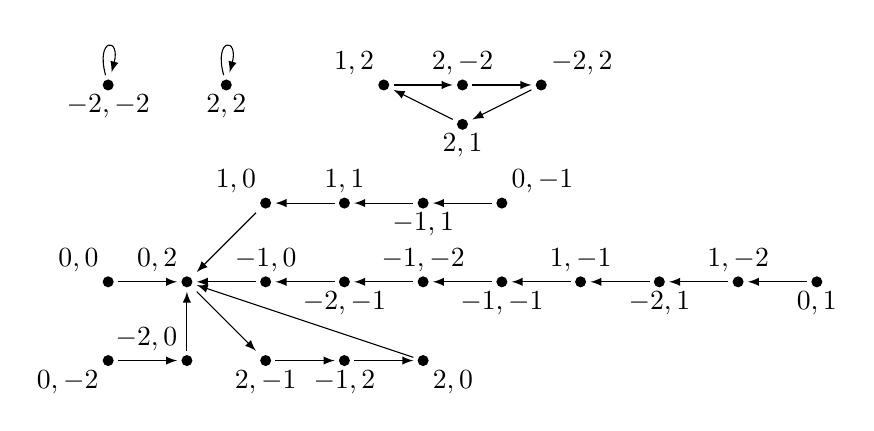
\begin{tikzpicture}[>=latex]
{\centering
\node (-2-2) at (-0.5, 2)    {};
\node (-2-1) at (2.5, -0.5)   {};
\node (-20) at (0.5, -1.5) {};
\node (-1-2) at (3.5, -0.5)   {};
\node (-1-1) at (4.5, -0.5) {};
\node (-10) at (1.5, -0.5)   {};
\node (0-2) at (-0.5, -1.5)   {};
\node (0-1) at (4.5, 0.5) {};
\node (00) at (-0.5, -0.5)    {};
\node (1-2) at (7.5, -0.5) {};
\node (1-1) at (5.5, -0.5)  {};
\node (10) at (1.5, 0.5) {};
\node (2-2) at (4, 2)   {};
\node (2-1) at (1.5, -1.5) {};
\node (20) at (3.5, -1.5) {};

\node (-22) at (5, 2)    {};
\node (-21) at (6.5, -0.5)  {};
\node (-12) at (2.5, -1.5)   {};
\node (-11) at (3.5, 0.5) {};
\node (02) at (0.5, -0.5)   {};
\node (01) at (8.5, -0.5) {};
\node (12) at (3, 2) {};
\node (11) at (2.5, 0.5)   {};
\node (22) at (1, 2)   {};
\node (21) at (4, 1.5) {};

\fill (-2-2)[right] circle (0.07) node[below]       {$-2,-2$};
\fill (-2-1)[right] circle (0.07) node[below]       {$-2,-1$};
\fill (-20)[left] circle (0.07) node[above left]       {$-2,0$};
\fill (-21)[left] circle (0.07) node[below]       {$-2,1$};
\fill (-22)[left] circle (0.07) node[above right]       {$-2,2$};
\fill (-1-2)[left] circle (0.07) node[above]       {$-1,-2$};
\fill (-1-1)[left] circle (0.07) node[below]  {$-1,-1$};
\fill (-10)[left] circle (0.07) node[above]       {$-1,0$};
\fill (-11)[left] circle (0.07) node[below]  {$-1,1$};
\fill (-12)[left] circle (0.07) node[below]  {$-1,2$};
\fill (0-2)[left] circle (0.07) node[below left]  {$0,-2$};
\fill (0-1)[left] circle (0.07) node[above right]       {$0,-1$};
\fill (00)[left] circle (0.07) node[above left]       {$0,0$};
\fill (01)[left] circle (0.07) node[below]  {$0,1$};
\fill (02)[left] circle (0.07) node[above left] {$0,2$};
\fill (2-2)[right] circle (0.07) node[above]       {$2,-2$};
\fill (2-1)[right] circle (0.07) node[below ]       {$2,-1$};
\fill (20)[left] circle (0.07) node[below right]       {$2,0$};
\fill (21)[left] circle (0.07) node[below]       {$2,1$};
\fill (22)[left] circle (0.07) node[below]       {$2,2$};
\fill (1-2)[left] circle (0.07) node[above]       {$1,-2$};
\fill (1-1)[left] circle (0.07) node[above]  {$1,-1$};
\fill (10)[left] circle (0.07) node[above left]       {$1,0$};
\fill (11)[left] circle (0.07) node[above]  {$1,1$};
\fill (12)[left] circle (0.07) node[above left]  {$1,2$};

%>>> def f(x1, x2):
%...     y = (x2 + 2 * x1 * x2 + 2) % 5
%...     return y if y < 3 else y - 5

%>>> d = {(x, y): (y, f(x, y)) for x in range(-2, 3) for y in range(-2, 3)}
%>>>for k in d:
%...     if k == d[k]:
%...             print('\path[->]', k, 'edge [loop above] node {} ();')
%...     else:
%...             print('\path[->]', k, 'edge node {}', d[k], ';')

\path[->] (-2-2) edge [loop above] node {} ();
\path[->] (-2-1) edge node {} (-10) ;
\path[->] (-20) edge node {} (02) ;
\path[->] (-21) edge node {} (1-1) ;
\path[->] (-22) edge node {} (21) ;
\path[->] (-1-2) edge node {} (-2-1) ;
\path[->] (-1-1) edge node {} (-1-2) ;
\path[->] (-10) edge node {} (02) ;
\path[->] (-11) edge node {} (11) ;
\path[->] (-12) edge node {} (20) ;
\path[->] (0-2) edge node {} (-20) ;
\path[->] (0-1) edge node {} (-11) ;
\path[->] (00) edge node {} (02) ;
\path[->] (01) edge node {} (1-2) ;
\path[->] (02) edge node {} (2-1) ;
\path[->] (1-2) edge node {} (-21) ;
\path[->] (1-1) edge node {} (-1-1) ;
\path[->] (10) edge node {} (02) ;
\path[->] (11) edge node {} (10) ;
\path[->] (12) edge node {} (2-2) ;
\path[->] (2-2) edge node {} (-22) ;
\path[->] (2-1) edge node {} (-12) ;
\path[->] (20) edge node {} (02) ;
\path[->] (21) edge node {} (12) ;
\path[->] (22) edge [loop above] node {} ();

}
\end{tikzpicture}

В случае $\gamma = (2, 2)$ последовательность оказывается полностью состоящей из двоек, поэтому период такой последовательности будет равен единице.

\task{Над полем $GF(2)$ построить ЛРП периода $T$ и ранга $n$ и указать начальное заполнение.

$T = 84, n = 8.$
}

Разложим $T$ на множители: $T = 84 = 4 \cdot 3 \cdot 7$. 

ЛРП$_1$ c периодом 4 соответствует минимальный многочлен
$$f_1 (x) = x^3 + x^2 + x + 1,\ x_i = x_{i-1} + x_{i-2} + x_{i-3}.$$

ЛРП$_2$ с периодом 3 соответствует минимальный многочлен
$$f_2 (x) = x^2 + x + 1,\ x_i = x_{i-1} + x_{i-2}.$$

ЛРП$_3$ с периодом 7 соответствует минимальный многочлен
$$f_3 (x) = x^3 + x + 1,\ x_i = x_{i-2} + x_{i-3}$$

Искомый характеристический многочлен
$$f(x) = (x^3 + x^2 + x + 1)(x^2 + x + 1)(x^3 + x + 1) = x^8 + x^4 + x^3 + x^2 + x + 1.$$

Характеристическое уравнение будет иметь вид:
$$x_i = x_{i-4} + x_{i-5} + x_{i-6} + x_{i-7} + x_{i-8}.$$

Выберем начальные заполнения для ЛРП$_{1-3}$, отличные от нуля, и получим первые начальные отрезки ЛРП длины $n=8$:
$$\widetilde \alpha _1 = 001 \Rightarrow \widetilde \beta _1 = 00110011$$
$$\widetilde \alpha _2 = 01 \Rightarrow \widetilde \beta _2  = 01101101$$
$$\widetilde \alpha _3 = 001 \Rightarrow \widetilde \beta _3 = 00101110$$

Искомое начальное заполнение:
$$\widetilde \beta = \widetilde \beta _1 \oplus \widetilde \beta _2 \oplus \widetilde \beta _3 = 01110000.$$

Ответ: $f(x) = x^8 + x^4 + x^3 + x^2 + x + 1$, $\widetilde \beta = 01110000$. 

\section{Перекрытия гаммы. Криптоанализ при неравновероятной гамме.}

\task{Два текста $x$ и $x'$ на русском языке зашифрованы шифром гамирования по $\mod 30$ с помощью одной и той же гаммы $\gamma$. Использована следующая таблица соответствия букв числами (здесь -- означает пробел): \\

\medskip
{\centering
\begin{tabular}{||c|c|c|c|c|c|c|c|c|c|c|c|c|c|c||}
\hline
А & Б & В & Г & Д & Е & Ж & З & И & К & Л & М & Н & О & П \\
\hline
00 & 01 & 02 & 03 & 04 & 05 & 06 & 07 & 08 & 09 & 10 & 11 & 12 & 13 & 14\\
\hline
Р & С & Т & У & Ф & Х & Ц & Ч & Ш & Щ & Ы & Э & Ю & Я & -- \\
\hline
15 & 16 & 17 & 18 & 19 & 20 & 21 & 22 & 23 & 24 & 25 & 26 & 27 & 28 & 29 \\
\hline
\end{tabular}

}
\medskip

Получено два шифротекста $y =$ КЛОВБЛЖЗФ и $y'=$ ВУПЗЕРСВЖ, известна тематика $x$ и $x'$: 'времена года'. Применяя 'протяжку вероятного слова' найти $x, x', \gamma$.

}

Переведём векторы $y$ и $y'$ в числа и найдём их разность:

\noindent $y - y' = x + \gamma - x' - \gamma = x - x' = (9 - 2, 10 - 18, 13 - 14, 2 - 7, 1 - 5, 10 - 15, \\ 6 - 16, 7 - 2, 19 - 6) = (7, 22, 29, 25, 26, 25, 20, 5, 13) = $ ЗЧ--ЫЭЫЧЕО.

Попробуем подставить в начало $x'$ слово 'ЗИМА--':

\noindent $x = (x - x') + x' = АСНЕГ * * * *$

Видно, что получается осмысленное предложение. Посмотрим, какая гамма:

$\gamma = y' - x' = ВВВВВ ****$

Предположим, что гамма состоит только из этих букв, продлим и получим окончательный ответ:

\noindent $x = ЗИМА-ИДЕТ$

\noindent $x' = АСНЕГОПАД$

\noindent $\gamma = ВВВВВВВВВ$

\task{Пусть в шифре гаммирования по mod 30 используется только 6 знаков гаммы \(\{17, 05, 02, 15, 08, 14\} \) (соответствие букв и чисел в таблице):

\medskip
{\centering
\begin{tabular}{||c|c|c|c|c|c|c|c|c|c|c|c|c|c|c||}
\hline
А & Б & В & Г & Д & Е & Ж & З & И & К & Л & М & Н & О & П \\
\hline
00 & 01 & 02 & 03 & 04 & 05 & 06 & 07 & 08 & 09 & 10 & 11 & 12 & 13 & 14\\
\hline
Р & С & Т & У & Ф & Х & Ц & Ч & Ш & Щ & Ы & Ъ & Э & Ю & Я  \\
\hline
15 & 16 & 17 & 18 & 19 & 20 & 21 & 22 & 23 & 24 & 25 & 26 & 27 & 28 & 29 \\
\hline
\end{tabular}

}
\medskip


Получен шифртекст $y =$ ШАССЧАТАИЦОС. Используя "зигзагообразное" чтение дешифровать открытый текст и восстановить гамму. \\
}

Составим таблицу из возможных результатов гаммирования:

\medskip

{\centering
\begin{tabular}{||c|c|c|c|c|c|c|c|c|c|c|c|c|c|c||}
\hline
17 & Ж & О & Я & Я & Е & \bf О & А & О & Ц & Д & Ъ & \bf Я \\
\hline
05 & У & Ы & М & М & \bf Т & Ы & Н & Ы & Г & С & \bf И & М \\
\hline
02 & Ц & Ю & П & \bf П & Х & Ю & Р & Ю & Ж & \bf Ф & М & П \\
\hline
15 & И & \bf Р & Б & Б & З & Р & В & \bf Р & Ш & Ж & Ю & Б \\
\hline
08 & Р & Ч & \bf И & И & П & Ч & К & Ч & \bf А & О & Е & И \\
\hline
14 & \bf К & С & В & В & И & С & \bf Г & С & Щ & З & Я & В \\
\hline
\end{tabular}
}
\medskip

Легко видеть, $x = $ КРИПТОГРАФИЯ, $\gamma = $ ПРИВЕТПРИВЕТ.

\section{Теория групп}

\task{Определить структуру группы $\mathbb{Z}^*_n$ , разложить её в прямое произведение циклических подгрупп и подсчитать число элементов различного порядка, $n = 84$.}

$|G| = \phi (84) = \phi (2^2) \cdot \phi (3) \cdot \phi (7) = (4 - 2)(3 - 1)(7 - 1) = 24 = 2^3 \cdot 3$.

\noindent Следовательно, $G \cong S_1(8) \times S_2 (3)$.

1.  Определим структуру примарной группы $S_1(8)$. Для этого нужно решить сравнение:

$$x^2 \equiv 1 \pmod{84}.$$

По КТО это равносильно следующей системе:

\begin{equation*}
	\begin{cases}
	x^2 \equiv 1 \pmod 3 \\
	x^2 \equiv 1 \pmod 4 \\
	x^2 \equiv 1 \pmod 7
	\end{cases}
\end{equation*}

$p = 3 = 4 \cdot 0 + 3 \Rightarrow \lege{1}{3} = 1$ -- два решения: $x_1 \equiv \pm 1^{0+1} \pmod 3$.

$p = 4 = 2^2,\ a = 1 \Rightarrow $ два решения: $x_2 = \pm 1 \pmod 4$.

$p = 7 = 4 \cdot 1 + 3 \Rightarrow \lege{1}{7} = 1$ -- два решения: $x_3 \equiv \pm 1^{1+1} \pmod 7$.

Общее решение системы по КТО будет равно:

\begin{multline*}
X = x_1 (4 \cdot 7)[(4 \cdot 7)^{-1} \pmod 3] + x_2 (3 \cdot 7)[(3 \cdot 7)^{-1} \pmod 4] + \\
+ x_3 (3 \cdot 4)[(3 \cdot 4)^{-1} \pmod 7] \pmod {84} =
28 x_1 + 21 x_2 + 36 x_3 \pmod {84}
\end{multline*}

Таким образом, множество элементов второго порядка группы $G$ это:

$$M_2 = \{13, 43, 55, 29, 41, 71, 83\}.$$

Обозначим за $A_i = \left\langle M_{2, i} \right\rangle $, где $M_{2, i}$ -- $i$-тый элемент множества $M_2$. Тогда $S_1(8) \cong A_i \times A_j \times A_k$, $i, j, k = \overline{1, 7} $.

2. Определим структуру примарной группы $S_2(3)$. Для этого нужно решить сравнение:

$$x^3 \equiv 1 \pmod{84}.$$

По КТО это равносильно следующей системе:

\begin{equation*}
	\begin{cases}
	x^3 \equiv 1 \pmod 3 \\
	x^3 \equiv 1 \pmod 4 \\
	x^3 \equiv 1 \pmod 7
	\end{cases}
\end{equation*}

Первые два сравнения, очевидно, имеют единственные решения $x_1 =~1$, $x_2 = 1$. Последнее сравнение имеет 3 решения: $x_3 = \{1, 2, 4\}$. Общее решение исходного сравнения будет равно:

$$X = 28 x_1 + 21 x_2 + 36 x_3 \pmod {84} = 49 + 36 x_3 \pmod {84}$$

Множество элементов третьего порядка группы $G$ это:

$$M_3 = \{25, 37\}$$

Таким образом, $S_2(3) = \left\langle 25 \right\rangle = \left\langle 37 \right\rangle$. \\

\noindent Ответ: $G \cong A_i \times A_j \times A_k \times \left\langle 25 \right\rangle = A_i \times A_j \times A_k \times \left\langle 37 \right\rangle$, $i, j, k = \overline{1, 7}$. 

\task{Доказать, что $y = x^3$ -- подстановка над $\mathbb{Z}_p$, если \\$p \equiv 2 \pmod{3}$, то есть, 
$$x_1^3 \equiv x_2^3 \pmod p \Rightarrow x_1 \equiv x_2 \pmod p.$$}

Поле $\mathbb{Z}_p$ имеет порядок $\phi(p) = p - 1$.
Из $x_1^3 \equiv x_2^3 \pmod p$ получим, что $(x_1 x_2 ^{-1})^3 \equiv 1 \pmod p$. Тогда порядок $x_1 x_2^{-1}$ является делителем $3$. Существует два варианта:

1. Ord($x_1 x_2^{-1}$) = 1. Это означает, что $x_1 \equiv x_2 \pmod p$.

2. Ord($x_1 x_2^{-1}$) = 3. Так как $p = 3m + 2$, то $\phi(p) = 3m + 1$. То есть, порядок элемента не является делителем порядка группы, что противоречит теореме Лагранжа.

Следовательно, $x_1 \equiv x_2 \pmod p$. А значит, $y = x^3$ -- подстановка над $\mathbb{Z}_p$.

\task{Найти порядок и цикловое представление подстановки $y~=~x^3,\ p = 11$.}

\medskip

\begin{tabular}{||c||c|c|c|c|c|c|c|c|c|c|c|}
 $x$ & 0 & 1 & 2 & 3 & 4 & 5 & 6 & 7 & 8 & 9 & 10 \\
 \hline
 $y$ & 0 & 1 & 8 & 5 & 9 & 4 & 7 & 2 & 6 & 3 & 10
\end{tabular}

\medskip

Получим 5 циклов: (0), (1), (2, 8, 6, 7), (3, 5, 4, 9), (10). Порядок подстановки равен НОК длины циклов: НОК$(1, 1, 4, 4, 1) = 4$.

Ответ: Порядок подстановки (0)(1)(2, 8, 6, 7)(3, 5, 4, 9)(10) равен 4.

\task{Найти порядок подстановки $y = 5 x + 3 \pmod {12}$}

\medskip

\begin{tabular}{||c||c|c|c|c|c|c|c|c|c|c|c|c|}
 $x$ & 0 & 1 & 2 & 3 & 4 & 5 & 6 & 7 & 8 & 9 & 10 & 11 \\
 \hline
 $y$ & 3 & 8 & 1 & 6 & 11 & 4 & 9 & 2 & 7 & 0 & 5 & 10
\end{tabular}

\medskip

Получим 3 цикла: (0, 3, 6, 9), (1, 8, 7, 2), (4, 11, 10, 5). Порядок подстановки равен НОК длины циклов: НОК$(4, 4, 4) = 4$.

Ответ: Порядок подстановки равен 4.

%\chapter{Экзамен}
\noindent \textit{1. Определение шифра. Шифр простой замены, перестановки, гаммирования. Основные условия криптоанализа.} \\

Отображение $T: X \times K \rightarrow Y$ называется \textbf{шифром}, если $\forall k \in K \\ \exists T^{-1} (y, k) = x$.

Пусть $A = \{ a_1, \ldots , a_m \}$ -- конечный алфавит, $S_m$ -- множество всех подстановок на $A$. Для некоторого натурального $n$ положим $X = A^n$. Если $x = (a_{i_1}, \ldots, a_{i_n})$, $k \in S_m$, то определим \textbf{шифр простой замены} следующим образом:
$$T(x, k) = (k(a_{i_1}), k(a_{i_2}), \ldots, k(a_{i_n})) = y = (b_{i_1}, \ldots, b_{i_n}).$$

Пусть $A = \{ a_1, \ldots , a_m \}$ -- конечный алфавит, $n$ -- натуральное число, $S_n$ -- симметрическая группа подстановок на множестве $\{1, \ldots, n\}$, $X =~A^n$. Если $x = (a_{i_1}, \ldots, a_{i_n})$, $k = \bigl(\begin{smallmatrix}
    1 & \cdots & n \\
    j_1 & \cdots & j_n
  \end{smallmatrix}\bigr) \in S_n$, то \textbf{шифр перестановки} на $X$ определяется следующим образом:
$$T(x, k) = (a_{i_{j_1}}, a_{i_{j_2}}, \ldots, a_{i_n}) = y.$$

Пусть $A = \{ 0, \ldots , m - 1 \}$ -- алфавит, $X =A^n$ -- множество открытых текстов. Рассмотрим кольцо вычетов $\mathbb{Z}_m$. Положим $K = A^n$ и $\forall x \in X, k \in K$, определим \textbf{шифр гаммирования}:
$$y = T(x, k) = (x + k) \pmod m,$$

\noindent где сложение происходит в кольце $\mathbb{Z}_m$.

\newpage
\textbf{Основные условия криптоанализа}:

\noindent 1. Известен шифртекст $y$, один или несколько. Задачи:

а) Нахождение $T$ -- преобразования зашифрования;

б) Нахождение $T, T^{-1}, x$ -- дешифрование по шифртексту.

\noindent 2. Известны одна или несколько пар $(x, y)$. Определить $T(T^{-1})$ и найти $k$ -- ключ шифрования.

\noindent 3. Известны $T(T^{-1})$, один или несколько шифртекстов y. Найти:

а) x -- бесключевое чтение;

б) k, x -- дешифрование по шифртексту при известной шифрсистеме.

\noindent 4. Известны $T, T^{-1}, (x, y)$. Найти $k$.

а) Известны особые x -- атака выбранного открытого текста;

а) Известны особые y -- атака с использованием шифртекста.

\noindent 5. Известны $T, T^{-1}$, шифртекст $y$ или пары $(x, y)$, некоторая форма преобразования $T(.,k)$, но неизвестны $k$ и $T^{-1}(., k)$ -- системы с открытым ключом (Диффи и Хеллман, 1976 г.) \\

\noindent \textit{2. Теоретическая стойкость по Шеннону. Практическая стойкость. Пример совершенного шифра.} \\

\textbf{Теоретическая стойкость} (совершенная секретность) -- Система является безопасной против атак противника с неограниченным временем и ресурсами.

\textbf{Практическая стойкость} (вычислительная) -- Система является безопасной против атак противника в ограниченный период времени с ограниченными ресурсами.

Шеннон определил совершенную секретность условием:
$$P(x | y) = P(x)\ \ \forall x \in X, y \in Y,$$
\noindent где $X, Y$ -- множества открытых сообщений и возможных шифртекстов.

\textbf{Пример совершенного шифра} -- шифр гаммирования, в котором равновероятный ключ имеет ту же длину, что и открытый текст. Пусть $X = \{0, 1\},\ Y = \{0, 1\}, K = \{0, 1\}$, $T(x, k) = (x \oplus k) \pmod 2$, \\ $T^{-1}(y, k) = (y \oplus k) \pmod 2$, $X \sim \begin{pmatrix}
    0 & 1 \\
    p & q
  \end{pmatrix}$, $q = 1 - p$, $Y \sim \begin{pmatrix}
    0 & 1 \\
    0.5 & 0.5
  \end{pmatrix}$, $K \sim \begin{pmatrix}
    0 & 1 \\
    0.5 & 0.5
  \end{pmatrix}$, $P(Y|X) = \frac{P(X, Y)}{P_X (X)} = \begin{pmatrix}
    y/x & 0 & 1 \\
    0 & 0.5 & 0.5 \\
    1 & 0.5 & 0.5 
  \end{pmatrix}$.

По формуле Байеса:
$$P(X = x | Y = y) = \frac{P_X(x) P(y | x)}{P(y)} = \frac{P_X(x)}{\frac{1}{2} 2} = P_X(x).$$

\noindent \textit{3. Метод полного перебора, его средняя трудоемкость. Параллельное опробование с помощью случайно выбираемого на каждом шагу ключа.} \\

Пусть известны $T, T^{-1}, (x, y)$, а ключ неизвестен. \textbf{Методом полного перебора} называется поиск решения уравнения $T(x, k) = y$ перебором по всем $k \in K,\ \ |K| < \infty$.

Определим случайные величины: $\tau$ -- количество опробований ключа включительно до момента обнаружения, $\xi_i = [$ключ на $i$-м месте$]$. Ключ равновероятен, тогда $P(\xi_i = 1) = \frac{1}{|K|}$ для всех $i = \overline{1, |K|}$. \textbf{Средняя трудоёмкость МПП}:
$$\mathbb{E} \tau = \sum_{i = 1}^{|K|} i P (\xi_i = 1)= \frac{1}{|K|} \sum_{i = 1}^{|K|} i = \frac{|K|(|K| + 1)}{|K| \cdot 2} = \frac{|K| + 1}{2}.$$

Пусть параллельно работают $N$ машин. Если $t$ -- число шагов работы машин, то $Nt$ -- число опробований. Число тактов опробования -- случайная величина $\eta$. Аналогом является задача о размещениях: в каждую из $|K|$ ячеек может попасть от $0$ до $N$ частиц. Вероятность того, что из комплекта $i$ ни одна частица не попадёт в данную ячейку, равна $q = (1 - \frac{1}{|K|})^N$. Первое попадание в данную ячейку на комплекте с номером $t$, означающее, что ключ получен, имеет вероятность $P(\eta = t) = q^{t-1}(1-q)$ -- с.в. $\eta$ имеет геометрическое распределение. Тогда \textbf{средняя трудоёмкость МПП при параллельном опробовании} равна: 
$$\mathbb{E}\eta = \frac{1}{1 - q} = \frac{1}{1 - (1 - \frac{1}{|K|})^N} \approx \big \{ N << |K| \big \} \approx \frac{1}{1 - 1 + \frac{N}{|K|}} = \frac{|K|}{N}.$$

\noindent \textit{4. Аналитический метод криптоанализа. Треугольные системы и их решение. Линейные системы. Сложность решения методом Гаусса.} \\

Пусть $K = K_1 \times K_2 \times \ldots \times K_r$, $x = (x_1 x_2 \ldots x_s)$, $y = (y_1 y_2 \ldots y_s)$, $x_i, y_i \in A$. \textbf{Идея аналитического метода} заключается в том, чтобы записать систему уравнений и решить её относительно ключа:

\begin{equation*}
    \begin{cases}
    y_1 = f_1 (x_1, \ldots, x_s, k_1, \ldots, k_r) \\
    \cdots \\
    y_s = f_s (x_1, \ldots, x_s, k_1, \ldots, k_r) 
    \end{cases}
\end{equation*}

\noindent Известны $f_i$ и $(x, y)$.

Пусть эту систему можно преобразовать к \textbf{треугольной системе}:

\begin{equation*}
    \begin{cases}
    g_1 (x, y) = h_1 (x, y, k_1) \\
    g_2 (x, y) = h_2 (x, y, k_1, k_2) \\
    \cdots \\
    g_r (x, y) = h_r (x, y, k_1, \ldots, k_r) 
    \end{cases}
\end{equation*}

\noindent 1. Опробуем $k_1 \in K_1$, число опробований $\le |K_1| \Rightarrow$ восстанавливаем $k_1$.

\noindent 2. Опробуем $k_2 \in K_2$, число опробований $\le |K_2| \Rightarrow$ восстанавливаем $k_2$.

\noindent \ldots

\noindent r. Опробуем $k_r \in K_r$, число опробований $\le |K_r| \Rightarrow$ восстанавливаем $k_r$. \\

\noindent Таким образом, сложность $\le |K_1| + |K_2| + \ldots + |K_r|$. \\

Пусть имеется \textbf{линейная система}:

\begin{equation*}
    \begin{cases}
    b_{11} k_1 + b_{12} k_2 + \ldots + b_{1r} k_r = g_1 (x, y)  \\
    b_{21} k_1 + b_{22} k_2 + \ldots + b_{2r} k_r = g_2 (x, y)  \\
    \cdots \\
    b_{r1} k_1 + b_{r2} k_2 + \ldots + b_{rr} k_r = g_r (x, y)  \\
    \end{cases}
\end{equation*}

\noindent Методом Гаусса решается за $\sum_{k=1}^r k^2 = \frac{r(r + 1)(2 r + 1)}{6} \approx \frac{r^3}{3}$ операций. \\

\noindent \textit{5. Регистр сдвига с нелинейной обратной связью. Линейная сложность. Условия регулярности (теорема с доказательством).} \\

Последовательность $\gamma$ называется \textbf{линейной рекуррентной последовательностью} (ЛРП) порядка $r > 0$ над $GF(2)$, если она описывается \textbf{законом рекурсии}:
$$\gamma_{n+r} = \sum_{i=0}^{r-1} \alpha_i \gamma_{n+i},\ \ n = 0,1,\ldots$$
\noindent $\alpha_i \in GF(2),\ i= \overline{0,r-1}$ и все операции выполняются в поле $GF(2)$.

\textbf{Нелинейная рекуррентная последовательность} (НЛРП) определяется выражением:
$$\gamma_{n+r} = f (\gamma_n, \gamma_{n+1}, \ldots, \gamma_{n+r-1}),\ \ n = 0,1,\ldots$$

\textbf{Регистр сдвига с нелинейной обратной связью} (НЛРС) выглядит следующим образом:

\medskip

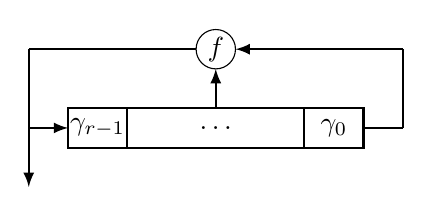
\begin{tikzpicture}[>=latex]
    {\centering
    
    \draw[thick] (0, 0) rectangle node[midway] {$\gamma_{r-1}$} (0.75, 0.5);

    \draw[thick] ( 0.75, 0) rectangle node[midway] {$\ldots$} (3 * 0.75 + 0.75, 0.5);
    \draw[thick, ->] (0.375 + 2 * 0.75, 0.5) -- (0.375 + 2 * 0.75, 1);

    \draw[thick] (4 * 0.75, 0) rectangle node[midway] {$\gamma_0$} (4 * 0.75 + 0.75, 0.5);

    \draw[thick, <-] (0,0.25) -- (-0.5,0.25);
    \draw[thick, <-] (-0.5, -0.5) -- (-0.5,1.25);
    \draw[thick, -] (-0.5,1.25) -- (1.875 - 0.25,1.25);
    
    \draw (1.875, 1.25) circle (0.25) node {$f$};
    
    \draw[thick, -] (3.75, 0.25) -- (4.25,0.25);
    \draw[thick, -] (4.25, 0.25) -- (4.25,1.25);
    \draw[thick, <-] (1.875 + 0.25,1.25) -- (4.25,1.25);

    }
\end{tikzpicture}

\medskip

Нелинейный регистр сдвига называется \textbf{регулярным}, если порождаемая им выходная последовательность $\gamma$ периодична при любом начальном заполнении регистра.

\textbf{Условие регулярности}: если НЛРС регулярен, то для любого начального заполнения существует ЛРС (вида) размера $v$ ($v \ge r$) такой, что порождаемая им последовательность совпадает с последовательностью, порождаемой при этом начальном заполнении НЛРС.

\prove{ НЛРС регулярен $\Rightarrow$ при любом начальном заполнении последовательность $\gamma$ периодична $\Rightarrow$ ЛРС вида $\gamma_{n+T} = \gamma_n,\\ n = 0, 1, \ldots$ порождает ту же последовательность.}

\noindent \textit{6. Метод “встреча посередине”. Трудоемкость метода. Пример реализации метода “встреча посередине”.} \\

Пусть даны два шифра: $T_1 (x, k_1)$ и $T_2 (z, k_2)$. Положим
$$y = T_2 (T_1 (x, k_1), k_2).$$

Ключ $k = (k_1, k_2)$, где $k_1 \in K_1,\ k_2 \in K_2,\ K = K_1 \times K_2$. Считаем, что в $T_1$ и $T_2$ согласованы области определения и области значений.

\textbf{Описание метода}. Пусть для пары $(x, y)$ существует единственный ключ. Составим две таблицы вида:
$$z_1 = T_1(x, k_1^{(1)}) \ldots \ldots z_{|K_1|} = T_1(x, k_1^{(|K_1|)}),$$
$$z'_1 = T^{-1}_2(y, k_2^{(1)}) \ldots \ldots z'_{|K_2|} = T^{-1}_2(y, k_2^{(|K_2|)}),$$

\noindent затем объединим их и упорядочим. Пара $z_i = z'_j$ определяет искомый ключ $k = (k_1^{(i)}, k_2^{(j)})$.

\textbf{Трудоёмкость метода}. Составление таблицы требует $|K_1|+|K_2|$ операций опробования. Упорядочивание таблицы размера $M$ оценивается в $M \ln M$ операций. Таким образом, средняя трудоёмкость метода равна:
$$(|K_1|+|K_2|)(1 + \ln {(|K_1|+|K_2|)}).$$
Если $|K| = N,\ |K_1| = |K_2|$, можно сделать такую оценку: $\sqrt{N} \ln N$.

\textbf{Пример}. Рассмотрим двойной $DES$ на ключах $k_1$ и $k_2$.

\medskip

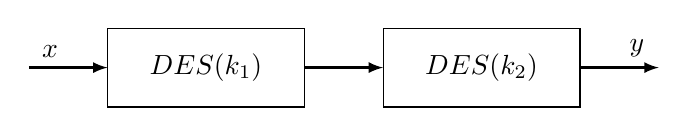
\begin{tikzpicture}[>=latex]
  {\centering
  \draw[thick, ->] (0,0) -- node[above left] {$x$} (1,0);
  \draw (1,-0.5) rectangle node[midway] {$DES(k_1)$} (3.5,0.5);
  \draw[thick, ->] (3.5,0) -- (4.5,0);
  \draw (4.5,-0.5) rectangle node[midway] {$DES(k_2)$} (7,0.5);
  \draw[thick, ->] (7,0) -- node[above right] {$y$} (8,0);
  }
\end{tikzpicture}

\medskip

Оценка трудоёмкости $2^{56} \ln 2^{112} \approx 10^{19} \ll 10^{34} \approx \frac{2^{56} \cdot 2^{56}}{2}$. Памяти потребуется $2N \approx 10^{17}$. \\

\noindent \textit{7. Метод “разделяй и побеждай”. Трудоемкость метода. Пример реализации метода.} \\

Ключ $k = (k_1, k_2)$, где $k_1 \in K_1,\ k_2 \in K_2,\ K = K_1 \times K_2$.

Пусть существует критерий $h$:

\begin{equation*}
h(x, y, k_1) = 
\begin{cases}
  1, & \exists k_2 \in K_2:\ T(x, (k_1, k_2)) = y \\
  0, & \forall k_2 \in K_2:\ T(x, (k_1, k_2)) \ne y
\end{cases}
\end{equation*}

Пусть известна пара $(x, y)$ достаточной длины, что $\exists ! k:\ T(x, k) = y$.

\textbf{Описание метода}. Первым шагом отбракуем элементы множества $K_1$, используя критерий $h$, и получим единственный $k_1$. На это потребуется $\frac{|K_1|}{2}$ опробований. На втором шаге применяем МПП относительно $k_2$, на это уйдёт $\frac{|K_2|}{2}$ опробований.

\textbf{Трудоёмкость метода} равна $\frac{|K_1| + |K_2|}{2}$.

\textbf{Пример}. Рассмотрим двойной $DES$ на ключах $k_1$ и $k_2$, устроенный таким образом, что открытый текст разбивается на блоки и каждый блок перед шифрованием складывается с предыдущим зашифрованным блоком. При этом каждый нечётный блок шифруется с использованием ключа $k_1$, а каждый чётный -- с $k_2$:
$$ОТ\ x = x_1 x_2 \ldots x_{2N},\ |x_i| = 64,\ i = \overline{1, 2N},$$
$$ШТ\ y = y_1 y_2 \ldots y_{2N},\ y_0 = 0,$$
$$DES(x_{2i+1} \oplus y_{2i}, k_1) = y_{2i+1},\ i = \overline{0, N-1},$$
$$DES(x_{2i} \oplus y_{2i-1}, k_2) = y_{2i},\ i = \overline{1, N}.$$
Пусть известна пара $(x, y)$. Получим следующие два множества:
$$A = \{(x_{2i+1} \oplus y_{2i}, y_{2i+1}),\ i = \overline{0, N-1},\ y_0 = 0\}$$
$$B = \{(x_{2i} \oplus y_{2i-1}, y_{2i}),\ i = \overline{1, N}\}$$
Определим критерий $h(x, y, k_1) = 1 \Leftrightarrow DES(x_{2i+1} \oplus y_{2i}, k_1) = y_{2i+1},\\ i = \overline{0, N-1}$.

Трудоёмкость метода составит $2^{56}$. \\

\noindent \textit{8. Методы криптоанализа при неравновероятной гамме.} \\

Пусть $x = x_1 x_2 \ldots x_n$ -- ОТ, $y = y_1 y_2 \ldots y_n$ -- ШТ, $\gamma = \gamma_1 \gamma_2 \ldots \gamma_n$ -- ключ, используется шифр гаммирования.

\textbf{Метод протяжки вероятностного слова}. Пусть для $(x, y)$ и $(x', y')$ использовался один и тот же ключ $\gamma$. Тогда:
$$y - y' = (x + \gamma) - (x' + \gamma) = x - x'.$$

\noindent Значит, если угадано (или предполагается), что начиная с некоторого места $i$ в $x$ стоит слово $a = a_1 a_2 \ldots a_r$, то в $x'$ на том же месте можно прочитать слово $a' = a'_1 a'_2 \ldots a'_r$, где $a'_j = y'_{i+j} - y_{i+j} + a_j$, $j = \overline{1, r}$.

\textbf{Метод чтения в колонках} (Зигзагообразное чтение). \\

Пусть всего используется $r$ значений гаммы. Составляется таблица, где в каждой строке находится сумма ШТ с некоторым значением гаммы $\gamma_i$. Всего таких строк $r$ штук. Криптоаналитик пытается восстановить ОТ, выбирая буквы из столбцов так, чтобы получался осмысленный читаемый текст.

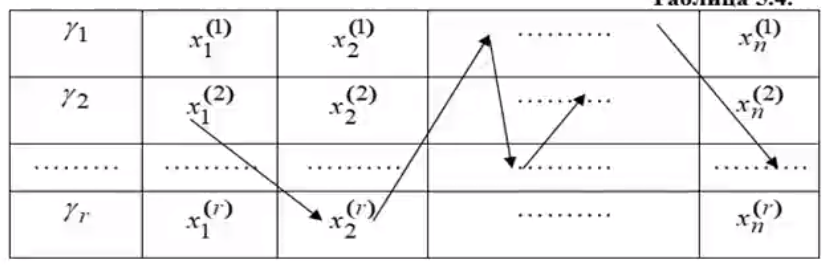
\includegraphics[scale=.5]{eka/img/zig_zag.png}

\noindent \textit{9. Первая теорема Шеннона (теорема с доказательством).} \\

Пусть $p(a_1) \ldots p(a_m)$ -- вероятности появления букв на фиксированном месте $i$ в открытом сообщении длины $n$. Предположим, что буквы в сообщении появляются независимо друг от друга с одним и тем же распределением. Обозначим через $\nu_i,\ i = \overline{1, m}$ частоты букв $a_1 \ldots a_m$ в последовательности $x$ (ОТ). Тогда вероятность выбора $x$ в нашей схеме равна
$$P(x) = p^{\nu_1}(a_1) \cdot \ldots \cdot p^{\nu_m}(a_m).$$
Будем считать, что $p(a_i) > 0,\ H = - \sum_{i=1}^m p(a_i) \log_2{p(a_i)}$.

\textbf{Теорема 1}. Для любых $\epsilon > 0 $ и $\delta > 0$ можно найти такое $n_0$, что для любого $n > n_0$ последовательности из $V_n$ распадаются на два непересекающихся класса $B$ и $\overline{B}$ так, что:
$$1) P(\overline{B}) < \epsilon$$
$$2) \Big |\frac{\log_2{P^{-1}(x)}}{n} - H \Big | < \delta,\ \forall x \in B$$

\prove{ Возьмём произвольные малые $\epsilon > 0 $ и $\delta > 0$ и рассмотрим события
$$\overline{B}_i = \{ x \in V_n, |\nu_i - np(a_i)| > \delta n \},\ i = \overline{1, m}.$$

Эти события означают, что в слове длины $n$ реальная частота встречаемости буквы $a_i$ отличается от её теоретической встречаемости больше, чем на $\delta n$.
Из ЗБЧ следует, что $\exists n^{(i)}_0:\ \forall n > n^{(i)}_0 \Rightarrow P(\overline{B}_i) < \frac{\epsilon}{m}$ (точнее, из неравенства Чебышёва: $P(|X - \mu| \ge k \sigma) \le \frac{1}{k^2}$). Определим $\overline B = \bigcup_{i=1}^m \overline B_i$. Тогда:
$$P(\overline B) = P(\bigcup_{i=1}^m \overline B_i) \le \sum_{i=1}^m P(\overline{B}_i) < \epsilon,\ \ \forall n > \max_i (n_0^{(i)}).$$

Первое утверждение доказано. Рассмотрим теперь следующее представление множества $B$:
$$B = \overline{\overline B} = \overline{\bigcup_{i=1}^m \overline B_i} = \bigcap_{i=1}^m \overline {\overline B}_i = \bigcap_{i=1}^m B_i,$$
$$B_i = \{ x \in V_n, |\nu_i - np(a_i)| \le \delta n \},\ i = \overline{1, m}.$$
Обозначим за $\alpha_i = \nu_i - np(a_i),\ i = \overline{1, m}$. Тогда $|\alpha_i| \le \delta n$. Выразим вероятность выбора ОТ через $\alpha_i$ (см. выражение перед теоремой):
$$P(x) = p^{\alpha_1 + np(a_1)}(a_1) \cdot \ldots \cdot p^{\alpha_m + np(a_m)}(a_m) = \prod_{i=1}^m p^{\alpha_i + np(a_i)}(a_i).$$
Тогда получим:
\begin{multline*}
\log_2 {\frac{1}{P(x)}} = \log_2 {\prod_{i=1}^m p^{- \alpha_i - np(a_i)}(a_i)} = - \sum_{i=1}^m (\alpha_i + np(a_i))\log_2 p(a_i) = \\
= - n \sum_{i=1}^m p(a_i) \log_2 p(a_i) - \sum_{i=1}^m \alpha_i \log_2 p(a_i) = n H - \sum_{i=1}^m \alpha_i \log_2 p(a_i)
\end{multline*}
Следовательно,
\begin{multline*}
\Big |\frac{\log_2{P^{-1}(x)}}{n} - H \Big | = \Big | - \frac{1}{n}\sum_{i=1}^m \alpha_i \log_2 p(a_i) \Big | \le \frac{1}{n} \sum_{i=1}^m | \alpha_i | | \log_2 p(a_i) | < \\
< \delta \sum_{i=1}^m | \log_2 p(a_i) | = \delta \cdot c
\end{multline*}
Поскольку $p(a_i) > 0$, сумма конечна и является константой (от $n$ не зависит).}

\noindent \textit{10. Вторая теорема Шеннона (теорема с доказательством).} \\

Упорядочим множество всех возможных последовательностей по убыванию вероятности возможности появления их в качестве открытого текста. Определим множество наиболее вероятных ОТ для $0 < \epsilon < 1$ таким образом:
$$Q_n(\epsilon) \subseteq V_n : P(Q_n(\epsilon)) \ge 1 - \epsilon,\ \forall y \in Q_n(\epsilon): P( Q_n(\epsilon) \setminus y) < 1 - \epsilon.$$
Обозначим $\beta_n (\epsilon) = | Q_n(\epsilon) |$.

Докажем, что множество $Q_n(\epsilon)$ содержит минимальное число последовательностей среди всех множеств $C$, таких что $P(C) \ge 1 - \epsilon$. 

От противного. Пусть $Q_n(\epsilon)$ -- не минимальное множество. Это означает $|C \setminus Q_n(\epsilon)| < | Q_n(\epsilon) \setminus C|$. По определению $Q_n(\epsilon)$, в нём содержатся наиболее вероятные последовательности. Тогда $\forall x \in Q_n(\epsilon), x \not \in C$ и $\forall y \not \in Q_n(\epsilon), y \in C$ справедливо $P(x) \ge P(y)$. Следовательно:
$$\sum_{y \in C \setminus Q_n(\epsilon)} P(y) < \sum_{x \in Q_n(\epsilon) \setminus C} P(x),$$
поскольку справа слагаемых хотя бы на 1 больше и все они не меньше слагаемых в левой сумме.

Пусть $x_0 = \underset{{x \in Q_n(\epsilon) \setminus C}}{\min} P(x)$. Значит,
$$P(C \setminus Q_n(\epsilon)) = \sum_{y \in C \setminus Q_n(\epsilon)} P(y) \le \sum_{x \in Q_n(\epsilon) \setminus (C \cup \{x_0\})} P(x) = P(Q_n(\epsilon) \setminus (C \cup \{x_0\})).$$
$$Q_n(\epsilon) \setminus \{x_0\} = (Q_n(\epsilon) \cap C) \cup ((Q_n(\epsilon) \setminus C) \setminus \{x_0\})\  (очев.)$$
$$P(Q_n(\epsilon) \setminus \{x_0\}) < 1 - \epsilon\ (опр.)$$
\begin{multline*}
P(C) = P(C \cap Q_n(\epsilon)) + P(C \setminus Q_n(\epsilon)) \le P(C \cap Q_n(\epsilon)) + \\
+ P(Q_n(\epsilon) \setminus (C \cup \{x_0\})) = P(Q_n(\epsilon) \setminus \{x_0\}) < 1 - \epsilon
\end{multline*}
Получили $P(C) < 1 - \epsilon$ -- противоречие, значит, $Q_n(\epsilon)$ -- минимальное множество.

\textbf{Теорема 2}. $\forall \epsilon > 0$
$$\lim_{n \rightarrow \infty} \frac{\log_2 {\beta_n (\epsilon)}}{n} = H$$

\prove{ Возьмём малое $\delta > 0$ и рассмотрим множество $B$ из первой теоремы Шеннона. Тогда, $\forall x \in B$ по этой теореме получим:
\begin{multline*}
\Big |\frac{\log_2{P^{-1}(x)}}{n} - H \Big | < \delta \Rightarrow H - \delta < \frac{-\log_2{P(x)}}{n} < H + \delta \Rightarrow \\
\Rightarrow -n(H + \delta) < \log_2{P(x)} < -n(H - \delta) \Rightarrow 2^{-n(H + \delta)} < P(x) < 2^{-n(H - \delta)}
\end{multline*}
Так как $B$ и $\overline B$ не пересекаются, можно записать:
\begin{multline*}
P(Q_n(\epsilon)) = \sum_{x \in Q_n(\epsilon)} P(x) = \sum_{x \in Q_n(\epsilon) \cap B} P(x) + \sum_{x \in Q_n(\epsilon) \cap \overline B} P(x) < \\
< \sum_{x \in Q_n(\epsilon) \cap B} 2^{-n(H - \delta)} + P(\overline B) = \big | Q_n(\epsilon) \cap B \big | 2^{-n(H - \delta)} + P(\overline B) < \\
< \big | Q_n(\epsilon) \big | 2^{-n(H - \delta)} + \epsilon = \beta_n (\epsilon) 2^{-n(H - \delta)} + \epsilon
\end{multline*}
По определению:
$$1 - \epsilon \le P(Q_n(\epsilon)) < \beta_n (\epsilon) 2^{-n(H - \delta)} + \epsilon \Rightarrow \beta_n (\epsilon) > 2^{n(H - \delta)} (1 - 2 \epsilon)$$
С другой стороны,
$$\beta_n(\epsilon) = | Q_n(\epsilon) | \le |B| = \sum_{x \in B} 1 < \sum_{x \in B} \frac{P(x)}{2^{-n(H + \delta)}} \le 2^{n(H + \delta)}$$
Тогда
$$2^{n(H - \delta)} < \beta_n(\epsilon) < 2^{n(H + \delta)} \Rightarrow H - \delta < \frac{\log_2 {\beta_n (\epsilon)}}{n} < H + \delta \Rightarrow$$
$$\Rightarrow \Big | \frac{\log_2 {\beta_n (\epsilon)}}{n} - H \Big | < \delta \Rightarrow \lim_{n \rightarrow \infty} \frac{\log_2 {\beta_n (\epsilon)}}{n} = H.$$}

\noindent \textit{11. Модель открытого текста, оценка числа открытых текстов.} \\

%\textbf{Модель открытого текста(?)}
%Используется шифр гаммирования по модулю $m$. Пусть $V_n$ -- слова длины $n$ в алфавите $\mathbb Z_m$. $X_n$ -- множество ОТ длины $n$, $Y_n$ -- множество ШТ длины $n$, $X_n, Y_n \subseteq V_n$. Пусть $\gamma$ принимает только $r$ значений. Тогда $\forall y \in Y_n$ соответствует $k = r^n$ различных $\{x^{(1)} \ldots x^{(k)} \} \subseteq V_n$ (именно $V_n$, потому что не все они являются ОТ). ШТ можно дешифровать однозначно, если $r = 1$. Однако если $r > 1$, то некоторый $x^{(i)}$ может не быть в множестве $X_n$. Как определить $r$, при которых возможно однозначное дешифрование?

%Пусть гамма выбирается равновероятно: $P(\gamma) = \frac{1}{|K|}$. Предположим также, что все $\{x^{(1)} \ldots x^{(k)} \}$, кроме исходного ОТ $x_0$, получены из некоторого $y$ случайно равновероятно: $P(y, x^{(j)}) = \frac{1}{m^n - 1}$ (предположение Шеннона в модели случайного шифра).

%Введём случайную величину
%$$\xi_i = 
%\begin{cases} 
%1, & x^{(i)} \in X_n \\
%0, & x^{(i)} \not \in X_n
%\end{cases}.$$
%Тогда число ложных ОТ $\eta$ среди $\{x^{(1)} \ldots x^{(k)} \} \setminus \{x_0\}$ равно:
%$$\eta = \sum_{i=1}^k \xi_i - 1,$$
%$$\mathbb E \eta = \sum_{i=1}^k \mathbb E \xi_i - 1.$$
%Так как
%$$\mathbb E \xi_i = 
%\begin{cases} 
%1, & x^{(i)} = x_0 \\
%\frac{|X|}{m^n - 1}, & x^{(i)} \ne x_0
%\end{cases},$$
%получим
%$$\mathbb E \eta = (k-1)\frac{|X|}{m^n - 1}.$$

\textbf{Модель открытого текста}. Пусть $p(a_1) \ldots p(a_m)$ -- вероятности появления букв на фиксированном месте $i$ в открытом сообщении длины $n$. Предположим, что буквы в сообщении появляются независимо друг от друга с одним и тем же распределением. Обозначим через $\nu_i,\ i = \overline{1, m}$ частоты букв $a_1 \ldots a_m$ в последовательности $x$ (ОТ). Тогда вероятность выбора $x$ в нашей схеме равна
$$P(x) = p^{\nu_1}(a_1) \cdot \ldots \cdot p^{\nu_m}(a_m).$$
Будем считать, что $p(a_i) > 0,\ H = - \sum_{i=1}^m p(a_i) \log_2{p(a_i)}$.

Возьмём произвольные малые $\epsilon > 0 $ и $\delta > 0$ и рассмотрим события
$$B_i = \{ x \in V_n, |\nu_i - np(a_i)| \le \delta n \},\ i = \overline{1, m},$$
$$\overline{B}_i = \{ x \in V_n, |\nu_i - np(a_i)| > \delta n \},\ i = \overline{1, m}.$$

\textbf{Оценка по теореме Шеннона}.
Множество ОТ можно представить как $X = B \cup \overline B$. Из первой теоремы Шеннона следует, что $\overline B$ имеет очень малую вероятность ($P(\overline B) \ll 1$). Из той же теоремы следует свойство равнораспределённости: для каждого $x \in B$ справедливо $P(x) \approx 2^{-nH}$. Таким образом, $|\overline B| \approx 0$ и $|B| \approx 2^{nH}$. Тогда число ОТ можно оценить как $|X| \approx 2^{nH}$. \\

\noindent \textit{12. Перекрытия гаммы. Средняя длина цикла с данной точкой в случайной подстановке.} \\

\textbf{Перекрытия гаммы}. Пусть $x = x_1 x_2 \ldots x_n$ -- ОТ, $y = y_1 y_2 \ldots y_n$ -- ШТ, $\gamma = \gamma_1 \gamma_2 \ldots \gamma_n$ -- ключ, используется шифр гаммирования. Есть две различные пары $(x, y)$ и $(x', y')$. Какова вероятность перекрытия?

Пусть $p(a_1) \ldots p(a_m)$ -- вероятности появления букв на фиксированном месте $i$ в открытом сообщении длины $n$ (распределение $P$). Тогда с.в. $\xi = x - x'$ имеет распределение $P^* = P*P$ -- свёртка $P$ с $P$.

В случае, если имеется перекрытие, получим $y - y' = x - x'$ -- имеет то же распределение $P^*$.

Если перекрытия нет, то $y-y' = (x - x') + (\gamma - \gamma')$. Поскольку гамма выбирается равновероятно, то $\gamma-\gamma'$ тоже имеет равновероятное распределение, а следовательно, и $y-y'$.

Пусть есть статистический критерий, проверяющий гипотезу $H_0$ о равновероятности $y-y'$ против альтернативы $H_1$, что $y-y'$ имеет распределение $P^*$. Тогда принятие гипотезы $H_0$ будет означать отсутствие перекрытия гаммы, а принятие $H_1$ -- наличие перекрытия.

\textbf{Средняя длина цикла с данной точкой в случайной подстановке}. Гамму получают с помощью конечного автомата $A$ без входа, в котором начальное состояние является ключом $k$. Из-за конечности множества состояний автомата обязательно возникнет период. Пусть $A$ -- равновероятная подстановка на множестве $\{1, \ldots , n\}$. Оценим количество шагов автомата до того, как он попадёт обратно в состояние $k$.

Пусть $t$ -- длина полученного цикла. Введём случайную величину

$$\xi_i = 
\begin{cases}
1, & t = i\\
0, & t \ne i
\end{cases}.
$$

Тогда $t = \sum_{i=1}^n i \xi_i$ и $\mathbb E t = \sum_{i=1}^n i \mathbb E \xi_i$.

Получим $P(\xi_i = 1)$. Для того, чтобы цикл был длины $i$, можно выбрать $i-1$ состояний случайным образом (начальное состояние фиксировано -- $k$) -- $C_{n-1}^{i-1}$, расположить их же случайным образом -- $(i-1)!$ и случайно расположить оставшиеся состояния -- $(n-i)!$. При этом всего различных автоматов (-перестановок) длины $n$  -- $n!$ штук.
$$P(\xi_i = 1) = \frac{C_{n-1}^{i-1} (i-1)! (n-i)!}{n!} = \frac{(n-1)! (i-1)! (n-i)!}{(i-1)! (n-i)! n!} = \frac{1}{n}$$
$$\mathbb E \xi_i = 1 \cdot P(\xi_i = 1) + 0 \cdot P(\xi_i = 0) = P(\xi_i = 1) = \frac{1}{n}$$

Следовательно,
$$\mathbb E t = \sum_{i=1}^n i \mathbb E \xi_i = \frac{1}{n} \sum_{i=1}^n i = \frac{1}{n} \cdot \frac{n(n+1)}{2} = \frac{n+1}{2}.$$ \\

\noindent \textit{13. Линейный криптоанализ блочных шифров.} \\

%Пусть $S \in \{0, 1 \}$ -- случайная величина, $P(S = 1) = p$, $\Delta(S) = |1 - 2p|$.

%\textbf{Лемма}. Пусть $S_1, \ldots , S_n$ - независимые бинарные случайные величины. Тогда $\Delta(S_1 \oplus \ldots \oplus S_n) = \prod_{i=1}^n \Delta(S_i)$.
%\prove {Если $S_1$ и $S_2$ независимы, то
%\begin{multline*}
%P(S_1 \oplus S_2 = 1) = P(S_1 = 1) P(S_2 = 0) + P(S_1 = 0) P(S_2 = 1) = \\
%= p_1 (1 - p_2) + (1 - p_1)p_2 = p_1 + p_2 - 2 p_1 p_2
%\end{multline*}
%\begin{multline*}
%  \Delta(S_1 \oplus S_2) = | 1 - 2 P(S_1 \oplus S_2 = 1) | = |1 - 2 p_1 - 2 p_2 + 4 p_1 p_2 |= \\
%  = |1 - 2 p_1| \cdot |1 - 2 p_2| = \Delta(S_1)\Delta (S_2)
%\end{multline*}
%Осталось заметить, что операция сложения по модулю 2 -- ассоциативная операция.
%}

Рассмотрим схему произвольного итеративного блочного шифра в $i$-ом раунде: $\vec Y(i) = E(\vec X(i), \vec K(i))$, где $E$ -- функция шифрования, $\vec X(i)$ -- блок открытого текста в $i$-ом раунде, $\vec Y (i)$ -- блок шифртекста, $\vec K(i)$ - подключ, используемый в $i$-ом раунде. $\vec Y (i), \vec X(i) \in V_n$, $\vec K (i) \in V_m$, n -- размер блока, m -- размер подключа.

Обозначим через $(\vec X, \vec \alpha) = X_1 \alpha_1 \oplus \ldots \oplus X_n \alpha_n = X_{i_1} \oplus \ldots \oplus X_{i_k} = \\ = X[i_1, \ldots ,i_k]$ -- скалярное произведение двоичных векторов $\vec X$ и $\vec \alpha$, где $(\alpha_{i_1}, \ldots , \alpha_{i_k})$ -- единичные координаты вектора $\vec \alpha$.

\textbf{Линейным статистическим аналогом нелинейной
функции~E} (ЛСА) называется случайная величина
$$S(i) = (\vec Y(i), \alpha(i)) \oplus (\vec X(i), \beta(i)) \oplus (\vec K(i), \gamma(i)),$$
для которой $P(S(i) = 1) = p \ne \frac{1}{2}$ для произвольного $\vec X(i)$.

$\Delta(S(i)) = |1 - 2p|$ -- \textbf{эффективность линейного стат. аналога}.

\textbf{Эффективным линейным статистическим аналогом} (ЭЛСА) называется линейный статистический аналог
$$S_{1 \ldots n} = (\vec X(1), \vec \alpha) \oplus (\vec Y(n), \vec \beta) \oplus \sum_{i=1}^n (\vec K(i), \vec \gamma (i))$$
из заданного множества с наибольшим $\Delta$. \\

\noindent \textbf{Задачи линейного криптоанализа:}

1. Найти ЭЛСА и вычислить его вероятность.

2. Определить несколько или все биты ключа с помощью ЭЛСА. \\

\noindent \textbf{Задача нахождения ЭЛСА для S-боксов DES}.
$\vec Y \in V_4$, $\vec X, \vec K \in V_6$. Нелинейная функция, реализующая S-бокс может быть записана в виде
$$\vec Y = F_a (\vec X \oplus \vec K),\ a = \overline {1, 8}$$
Пусть $1 \le i < 64$, $1 \le j < 16$, а $\vec k$ -- двоичное представление числа $k \in \mathbb N$. ЛСА для каждого из таких уравнений будет уравнение вида
$$(\vec Y, \vec j) = (\vec X \oplus \vec K, \vec i).$$
Обозначим через $S_a(i, j)$ число ненулевых $\vec X \in V_6$ для $a$-го S-бокса DES таких, что выполняется указанное уравнение. Пусть
$$S^*_a(i^*, j^*):\ |S^*_a(i^*, j^*) - 32| = \underset{1 \le i < 64, 1 \le j < 16}{\max} |S_a(i, j) - 32|.$$
Тогда уравнение
$$(\vec Y, \vec j^*) = (\vec X \oplus \vec K, \vec i^*)$$
является ЭЛСА $a$-го S-бокса в классе всех ЛСА указанного вида с вероятностью
$$p_a = \frac{S^*_a(i^*, j^*)}{64}.$$ \\

\noindent \textit{14. Дифференциальный криптоанализ блочных шифров.} \\

Пусть есть схема блочного шифра, состоящая из $r$ блоков длины $N$, где выход одного блока соединяется с входом другого, ключи $\vec Z = (Z(1), \ldots Z(r))$ получаются по некоторой схеме из $Z_0$ или выбираются независимо равновероятно.
Пусть $X(1), X^*(1)$ -- пара ОТ, $Y(i), Y^*(i)$ -- соответствующие им ШТ на $i$-том цикле,
$$\Delta Х(1) = X(1) - X^*(1)$$
$$\Delta Y(i) = Y(i) - Y^*(i)$$

\textbf{Идея дифференциального криптоанализа} заключается в том, чтобы найти такие $\Delta Х(1)$, что при случайном равновероятном выборе $Х(1), Z(1), \ldots, Z(r-1)$ с вероятностью более $\frac{1}{2^N}$ появится $\Delta Y( r-1)$.

Преобразование $f$ называется \textbf{криптографически
слабым}, если по $\Delta Y(r-1), Y(r)$ и $Y^* (r)$ для некоторого (малого) числа пар $(Х(1), Х^* (1))$ можно найти (хотя бы часть) $Z(r)$.

Пара $(\alpha, \beta)$ возможных значений вектора $(\Delta X(1), \Delta Y(i))$ называется \textbf{дифференциалом $i$-го цикла}. \\

\noindent Пусть $f$ определяет операции в $\Delta$ и $f$ криптографически слаба. Тогда возможна следующая атака.

1. Выбираем дифференциал $(r-1)$-го цикла $(\alpha, \beta)$, для которого вероятность $Р(\Delta Y(r-1) = \beta\ |\ \Delta X(1) = \alpha)$ большая.

2. Случайно выбираем $X(1)$ и подбираем $X^* (1)$, чтобы
$\Delta X(1) = \alpha$. Пусть известны $Y(r)$ и $Y^* (r)$.

3. Делаем предположение, что $\Delta Y(r-1) = \beta$ и, зная $Y(r)$ и $Y^* (r)$, находим $Z(r)$.

4. Повторяем 2 и 3, пока один (частичный) ключ не начнет
появляться чаще других. Это и будет $Z(r)$.

5. Повторяем 1-4 до нахождения полного ключа. \\

\noindent \textit{15. Метод коллизий для хэш-функций (теорема с доказательством).} \\

Пусть $A = \{a_1, \ldots, a_m \}$ -- алфавит, $A^*$ - множество слов конечной длины в алфавите $A$. Пусть $H:\ A^* \rightarrow A^l$ -- хэш-функция. $N = |A^l|$.

Используется задача о днях рождения. Пусть у злоумышленника есть два сообщения: $M$ -- то, которое жертва подпишет, и $M'$ -- то, которое злоумышленнику нужно подписать. Варьируя стилем, шрифтом, интервалами и т.д. получаем $n$ различных вариантов каждого из сообщений с сохранением смысла. Затем, просматривая пары, злумышленник ищет совпадение:
$$H(M_i) = H(M'_j),\ i = \overline{1, n},\ j = \overline{1, n}$$

\textbf{Теорема}. Пусть $N, n \rightarrow \infty$, но $\frac{n^2}{N} \rightarrow t > 0$, тогда: $$p = (1 - e^{-t})(1 + o(1)).$$
\prove{
Найдём вероятность того, что при наборе из $n$ таких пар не окажется ни одного совпадения. Мы выбираем $n$ хэшей $H(M_i)$ из множества $A^l$ ($C_N^n$ вариантов). Поскольку нет ни одного совпадения, то по правой стороне выбираем $n$ хэшей из множества $A^l \setminus \{H(M_1), \ldots, H(M_n) \}$ ($C_{N-n}^n$ вариантов). Всего возможных вариантов выбора $(C_N^n)^2$. Таким образом,
$$1 - p = \frac{C_N^n C_{N-n}^n}{(C_N^n)^2} = \frac{(N-n)! n! (N-n)!}{n! (N - 2n)! N!} = \frac{\left[ (N-n)! \right] ^ 2}{N! (N-2n)!}.$$
Используем формулу Стирлинга:
\begin{multline*}
1 - p = \frac{\left[ (N-n)! \right] ^ 2}{N! (N-2n)!} = \\ =\frac{\left[ \left( \frac{N-n}{e} \right) ^ {N-n} \sqrt{2\pi(N-n)} \right] ^ 2 (1 + o(1))}{\left( \frac{N}{e} \right) ^ {N} \sqrt{2\pi N} \left( \frac{N-2n}{e} \right) ^ {N-2n} \sqrt{2\pi(N-2n)} (1 + o(1))} = \\
= \frac{(1 - \frac{n}{N})^{2N - 2n}}{(1 - \frac{2n}{N})^{N - 2n}} (1 + o(1))
\end{multline*}

Отсюда, используя разложение логарифма в ряд:
\begin{multline*}
  \ln{(1 - p)} = [(2N - 2n)\ln{(1 - \frac{n}{N})} - (N-2n) \ln{(1 - \frac{2n}{N})}](1 + o(1)) = \\
= [(2N - 2n)(- \frac{n}{N} - \frac{n^2}{2N^2} + O(\frac{n^3}{N^3})) - (N-2n) (- \frac{2n}{N} - \frac{2n^2}{N^2} + O(\frac{n^3}{N^3}))](1 + o(1)) = \\
= - \frac{n^2}{N} (1 + o(1)) = -t (1 + o(1))
\end{multline*}
Следовательно,
$$1 - p = e^{-t} (1 + o(1)),$$
$$p = (1 - e^{-t}) (1 + o(1)).$$
}

\noindent \textit{16-20. Атаки на тройной DES.} \\

\textbf{Режимы использования DES}.

\noindent Режим электронной кодовой книги (ECB -- Electronic Codebook): \\

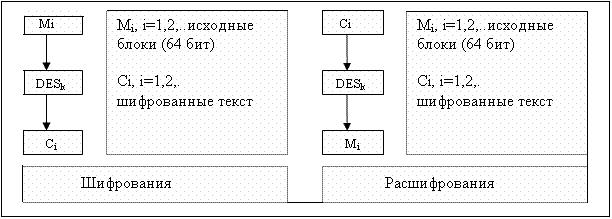
\includegraphics{eka/img/ECB.jpeg} \\

\noindent Режим сцепления блоков шифротекста (CBC -- Cipher Block Chaining): \\

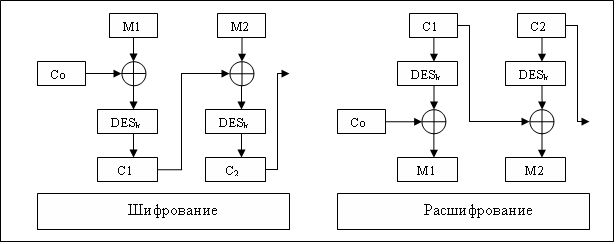
\includegraphics{eka/img/CBC.png} \\

\noindent Режим обратной связи по шифротексту (CFB -- Cipher Feedback): \\

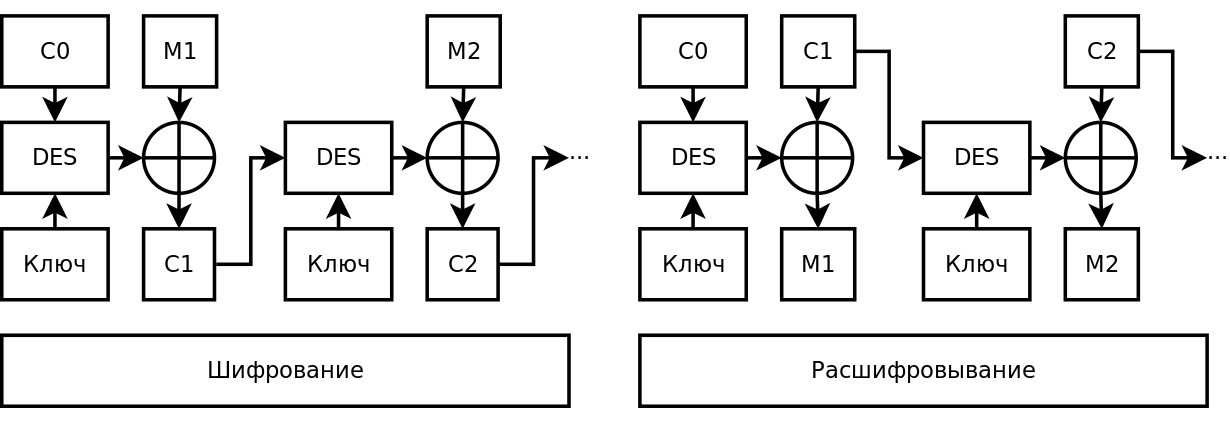
\includegraphics[scale=.3]{eka/img/CFB.png} \\

\noindent Режим обратной связи по выходу (OFB -- Output Feedback): \\

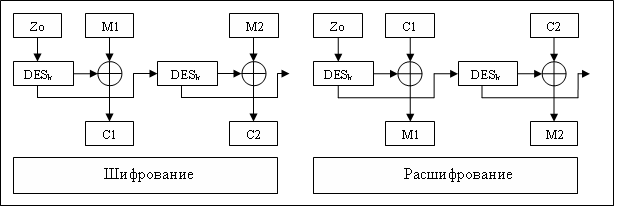
\includegraphics{eka/img/OFB.png} \\

\newpage
\noindent \textit{16. Атака на тройной DES в режиме CBC/CBC/ECB.} \\

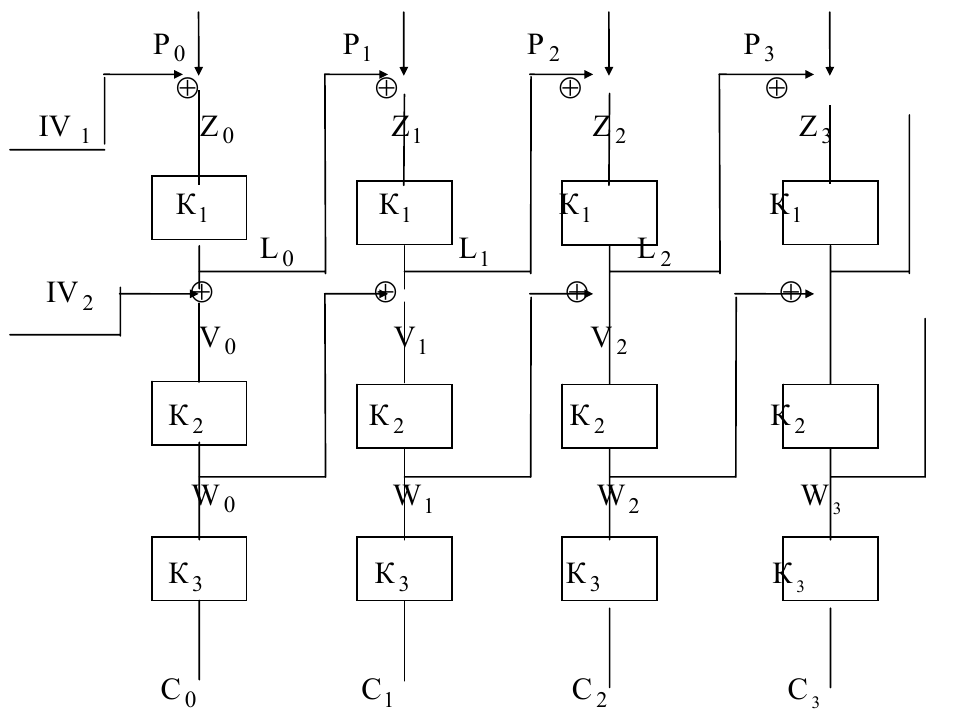
\includegraphics[scale=.4]{eka/img/CBC_CBC_ECB.png} \\

Используется атака выбранного шифротекста. Сначала будем искать ключ $K_3$. Среди всех ШТ выберем две тройки блоков следующего вида: $(C_0, C_1, C_2)$ и $(C_0^*, C_1, C_2)$, где $C_0 \ne C_0^*$.

Для первой тройки обозначим за $Z_i, V_i, W_i$ -- входы первого, второго и третьего блоков соответственно, $L_i$ -- выход первого блока, $P_i$ -- ОТ. Те же обозначения для второй тройки со звездочкой: $Z_i^*, V_i^*, W_i^*, L_i^*, P_i^*$.

Так как $C_1 = C_1^*, C_2 = C_2^*$, то $W_1 = W_1^*, W_2 = W_2^*, V_1 = V_1^*, V_2 = V_2^*$. Тогда $L_2 = L_2^*$ и $Z_2 = Z_2^*$.
Видно, что
$$W_0 \oplus L_1 = V_1,\ W_0^* \oplus L_1^* = V_1^* \Rightarrow W_0 \oplus W_0^* = L_1 \oplus L_1^*$$
$$P_2 \oplus L_1 = Z_2,\ P_2^* \oplus L_1^* = Z_2^* \Rightarrow P_2 \oplus P_2^* = L_1 \oplus L_1^*$$

Окончательно получим:
$$P_2 \oplus P_2^* = W_0 \oplus W_0^* = DES_{K_3}^{-1}(C_0) \oplus DES_{K_3}^{-1}(C_0^*)$$

Поскольку мы выбрали ШТ (а значит, знаем ОТ), мы можем совершить $2^{55}$ опробований в среднем, чтобы получить $K_3$.

Вероятность найти $C_1 = C_1^*, C_2 = C_2^*$ равна $\frac{1}{2^{128}}$. А значит, по задаче о днях рождения вероятность хоть какой-нибудь пары $\sqrt \frac{1}{2^{128}} = \frac{1}{2^{64}}$. Тогда потребуется $2^{64}$ блоков ШТ.

Для извлечения всего ключа требуется $3 * 2^{55}$ операций опробования и $3 * 2^{64}$ блоков ШТ. \\

\noindent \textit{17. Атака на тройной DES в режиме CBC/ECB/CBC.} \\

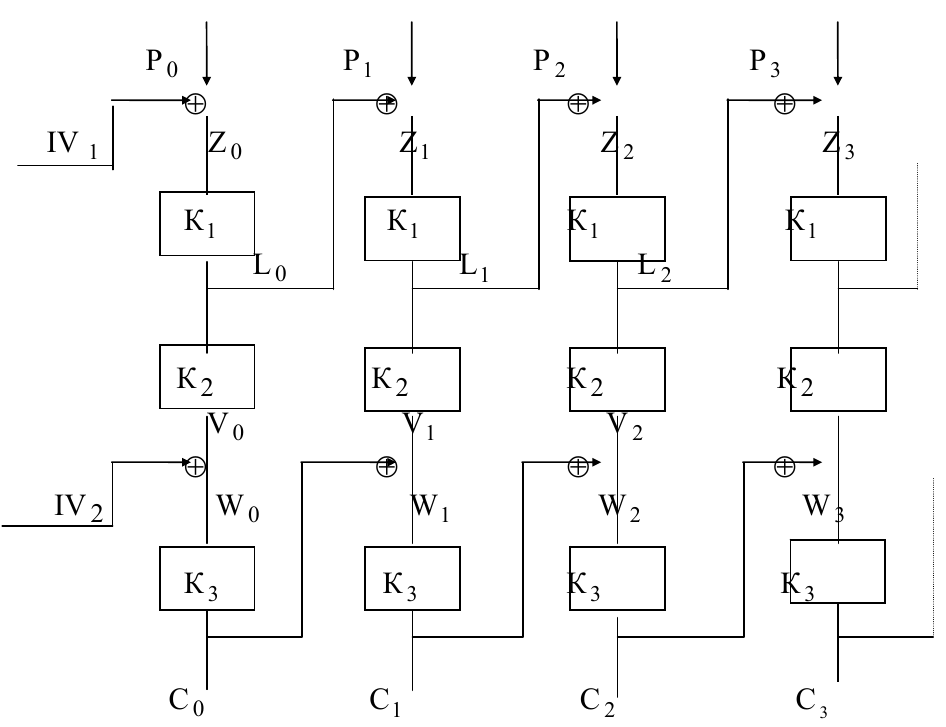
\includegraphics[scale=.4]{eka/img/CBC_ECB_CBC.png} \\

Используется линейный криптоанализ. Пусть найдено достаточно много шифртекстов $(C_0, C_1, C_2)$, где $C_1$ и $C_2$ фиксированы, а $C_0$ произвольные и различные.

1. Ищем $K_2$. Можно заметить, что $W_1 = C_0 \oplus V_1,\ V_1 = DES_{K_2}(L_1)$. Тогда $L_1 = DES_{K_2}^{-1}(C_0 \oplus W_1)$. Учитывая $L_1 \oplus P_2 = Z_2$, получим
$$P_2 = DES_{K_2}^{-1}(C_0 \oplus W_1) \oplus Z_2$$
Пусть $D*$ -- ЛСА $DES_{K_2}^{-1}$. Тогда, набрав достаточно уравнений, статистически выделим решение $K_2, W_1$ и $Z_2$.

2. Ищем $K_3$. С помощью МПП $DES_{K_3}(W_1) = C_1$.

3. Ищем $K_1$. Получим $L_1$:
$$L_2 = DES_{K_2}^{-1}(C_1 \oplus W_2) = DES_{K_2}^{-1}(C_1 \oplus DES_{K_3}^{-1}(C_2))$$
И далее МПП $DES_{K_1}(Z_2) = L_2$. \\

\newpage
\noindent \textit{18. Атака на тройной DES в режиме CBC/CBC/CBC.} \\

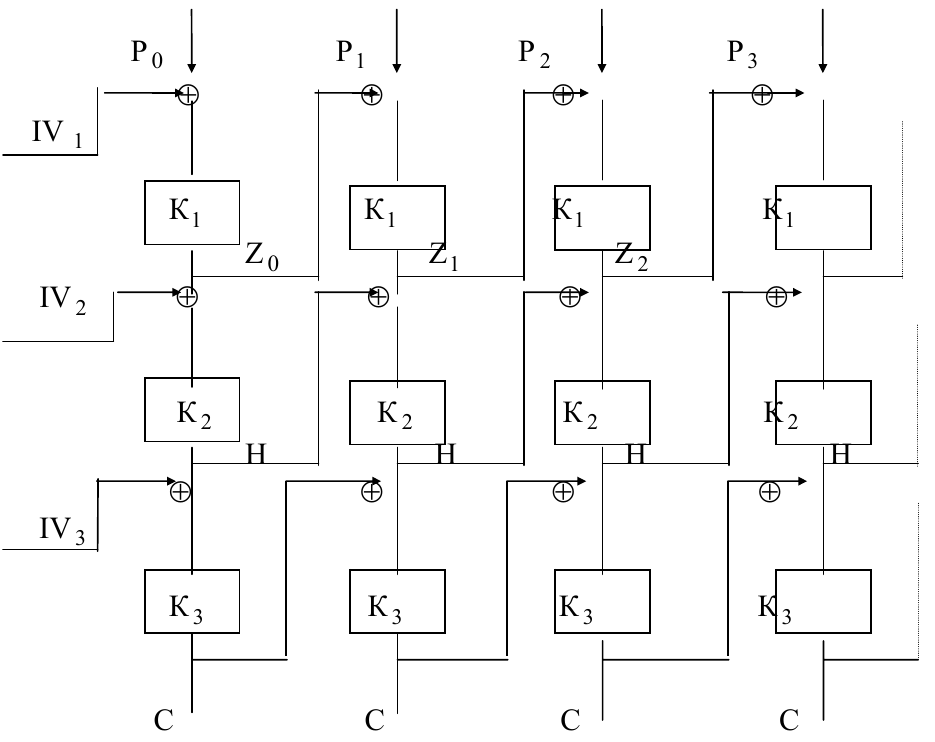
\includegraphics[scale=.4]{eka/img/CBC_CBC_CBC.png} \\

Атака, основанная на задаче о днях рождения. Пусть найдено $2^33$ шифртекстов вида $(C, C, C, С)$. Сначала ищем $K_3$.

На выходе второго блока имеем $(?, H, H, H)$, где $H = C + DES_{K_3}^{-1}(C)$. $H$ -- не взаимно-однозначное отображение, тогда для одного и того же $H$ с большой вероятностью (по задаче о днях рождения) найдутся различные $C$ и $C^*$, при этом у них будет один и тот же $P_3$:
$$Z_2 = H \oplus DES_{K_2}^{-1}(H)$$
$$DES_{K_1}(P_3 \oplus Z_2) = H \oplus DES_{K_2}^{-1}(H)$$
Тогда
$$P_3 = DES_{K_1}^{-1}(H \oplus DES_{K_2}^{-1}(H)) \oplus DES_{K_2}^{-1}(H) \oplus H$$
Для такой пары $C$, $C^*$ получим уравнение:
$$C + DES_{K_3}^{-1}(C) = C^* + DES_{K_3}^{-1}(C^*)$$
Решив его МПП, получим $K_3$. Аналогично остальные ключи.

\newpage
\noindent \textit{19. Атака на тройной DES в режиме ECB/CBC/CBC.} \\

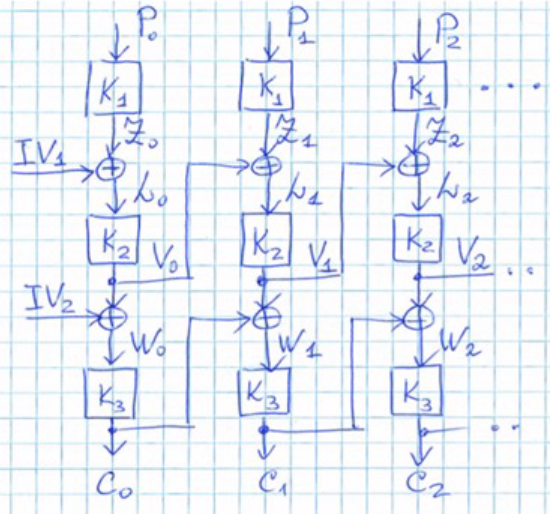
\includegraphics[scale=.5]{eka/img/ECB_CBC_CBC.png} \\

Атака использует дифференциальный криптоанализ. Сначала будем искать ключ $K_1$. Среди всех ШТ выберем две тройки блоков следующего вида: $(C_0, C_1, C_2)$ и $(C_0^*, C_1, C_2)$, где $C_0 \ne C_0^*$. Пусть $\Delta = C_0 \oplus C_0^*$.

Для первой тройки обозначим за $Z_i, V_i, W_i$ -- входы первого, второго и третьего блоков соответственно, $L_i$ -- выход первого блока, $P_i$ -- ОТ. Те же обозначения для второй тройки со звездочкой: $Z_i^*, V_i^*, W_i^*, L_i^*, P_i^*$.

Так как $C_1 = C_1^*, C_2 = C_2^*$, то $W_1 = W_1^*, W_2 = W_2^*, V_2 = V_2^*, L_2 = L_2^*$.
Тогда
$$V_1 = C_0 \oplus DES_{K_3}^{-1}(C_1), V_1^* = C_0 \oplus \Delta \oplus DES_{K_3}^{-1}(C_1) \Rightarrow V_1^* = V_1 \oplus \Delta$$
$$Z_2 = L_2 + V_1,\ Z_2^* = L_2^* + V_1^* \Rightarrow Z_2^* = Z_2 \oplus \Delta$$
Далее находим $K_1$, используя дифференциальный криптоанализ из
$$DES_{K_1}(P_2) \oplus DES_{K_1}(P_2^*) = C_0 \oplus C_0^*$$
Затем последовательно находим остальные ключи. \\

\newpage
\noindent \textit{20. Атака на тройной DES в режиме ECB/ECB/OFB.} \\

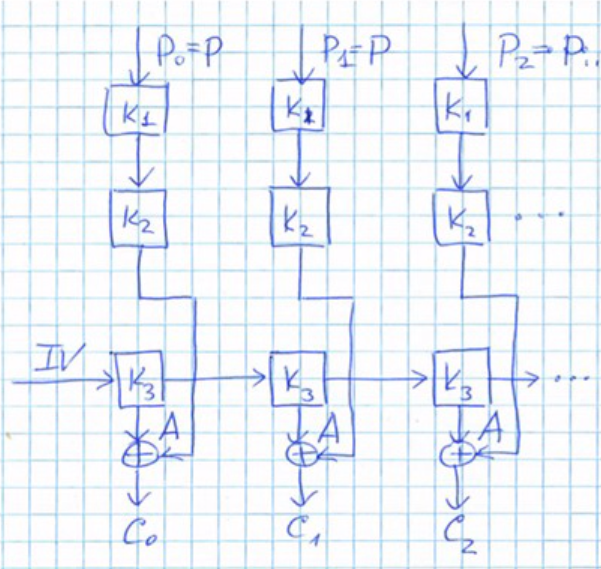
\includegraphics[scale=.5]{eka/img/ECB_ECB_OFB.png} \\

Сначала ищем ключ $K_3$. Выбираем произвольное $\vec P = (P, \ldots, P)$ из $2^{64}$ одинаковых блоков, пусть ему соответствует $C = (C_0, \ldots, C_{2^{64}-1})$. Период режима OFB $\le 2^{64}$.
Обозначим $A = DES_{K_2}(DES_{K_1}(P))$ и поток OFB $= v_0,\ldots,v_{2^{64}-1}$. Тогда $C_i = v_i \oplus A$. Таким образом, можно найти разности OFB-блоков:
$$C_0 \oplus C_1 = v_0 \oplus v_1, \ldots, C_{2^{64}-2} \oplus C_{2^{64}-1} = v_{2^{64}-2} \oplus v_{2^{64}-1}$$

1. Выбираем произвольное $u_0 = v_i$.

2. Перебирая $K$, вычисляем $u_1 = DES_{K}(u_0),\ u_2 = DES_{K}(u_1)$. Далее находим $u_0 \oplus u_1,\ u_1 \oplus u_2$, расположенные последовательно, в указанном выше ряде. Если такой пары нет, то либо $K \ne K_3$, либо $u_0$ не принадлежит периоду OFB. Перебрав все $K$, но не найдя такой пары, меняем $u_0$. Ожидается, что опробований $u_0$ будет $~2^{64}/$порядок OFB.

3. Как только нашли такие $u_0$ и $K$: $K_3 = K$, $v_i = u_0$, $v_{i+1} = u_1$. Получаем весь цикл OFB, что даёт нам возможность атаковать двойной DES в режиме ECB методом "встречи посередине".

\textbf{Сложность атаки}: Кол-во ОТ/кол-во шагов/память = $2^{64}/2^{58}/2^{56}$.

\end{document}